% https://github.com/martinhelso/UiB
%%%%%%%%%%%%%%%%%%%%%%%%%%%%%%%%%%%%%%%%%%%%%%%%%%%%%%%%%%%%%%%%%% - DOC SETTINGS
\documentclass[UKenglish,aspectratio=169]{beamer}
%%%%%%%%%%%%%%%%%%%%%%%%%%%%%%%%%%%%%%%%%%%%%%%%%%%%%%%%%%%%%%%%%% - THEME
\usetheme{UiB}
%%%%%%%%%%%%%%%%%%%%%%%%%%%%%%%%%%%%%%%%%%%%%%%%%%%%%%%%%%%%%%%%%% - PACKAGES
\usepackage[utf8]{inputenx} % For æ, ø, å
\usepackage{csquotes}       % Quotation marks
\usepackage{microtype}      % Improved typography
\usepackage{amssymb}        % Mathematical symbols
\usepackage{mathtools}      % Mathematical symbols
\usepackage[absolute, overlay]{textpos} % Arbitrary placement
\setlength{\TPHorizModule}{\paperwidth} % Textpos units
\setlength{\TPVertModule}{\paperheight} % Textpos units
\usepackage{tikz}
\usetikzlibrary{overlay-beamer-styles}  % Overlay effects for TikZ
\usepackage{graphicx}
\usepackage{multicol}
\usepackage{tabularx}
\usepackage[table]{xcolor}
\usepackage{pdfpages}
\usepackage{listings}
\usepackage{xcolor}
\usepackage{eso-pic}
%%%%%%%%%%%%%%%%%%%%%%%%%%%%%%%%%%%%%%%%%%%%%%%%%%%%%%%%%%%%%%%%%% - CUSTOM COLORS
\definecolor{codegreen}{rgb}{0,0.6,0}
\definecolor{codegray}{rgb}{0.5,0.5,0.5}
\definecolor{codepurple}{rgb}{0.58,0,0.82}
\definecolor{backcolour}{rgb}{0.95,0.95,0.92}
% Define colors
\definecolor{uiblightgreen}{HTML}{d8f3dc} % Light green for year
\definecolor{uibdarkgreen}{HTML}{83c5be} % Darker green for text
%%%%%%%%%%%%%%%%%%%%%%%%%%%%%%%%%%%%%%%%%%%%%%%%%%%%%%%%%%%%%%%%%% - DECKBLJAT
\author{Eduard Belan}
\title{pgx Service Desk}
\subtitle{Projektpräsentation}
\date{13. Januar 2025}



%%%%%%%%%%%%%%%%%%%%%%%%%%%%%%%%%%%%%%%%%%%%%%%%%%%%%%%%%%%%%%%%%% - DOC START
\begin{document}
% \hidelogo - logo only on frontpage - \showlogo shows logo on all pages
\hidelogo
%%%%%%%%%%%%%%%%%%%%%%%%%%%%%%%%%%%%%%%%%%%%%%%%%%%%%%%%%%%%%%%%%%%% - KAP.1
% Kap.1 - Einführung
\section{Einführung}
\begin{frame}{Inhaltsverzeichnis}
  \vspace{3em}
  \hspace{1em}
  \begin{minipage}{0.48\textwidth}
    {\small
      \tableofcontents[sections={1-3}]
    }
  \end{minipage}
  \hfill
  \begin{minipage}{0.48\textwidth}
    {\small
      \tableofcontents[sections={4-7}]
    }
  \end{minipage}
\end{frame}
%%%%%%%%%%%%%%%%%%%%%%%%%%%%%%%%%%%%%%%%%%%%%%%%%%%%%%%%%%%%%%%%%% - KAP.1.1
% Kap.1 - Einführung - About Me - 1.1
\subsection{About Me}
\SubSectionPage
\begin{frame}{Hochschule Pforzheim - Wirtschaftsinformatik}
  \centering
    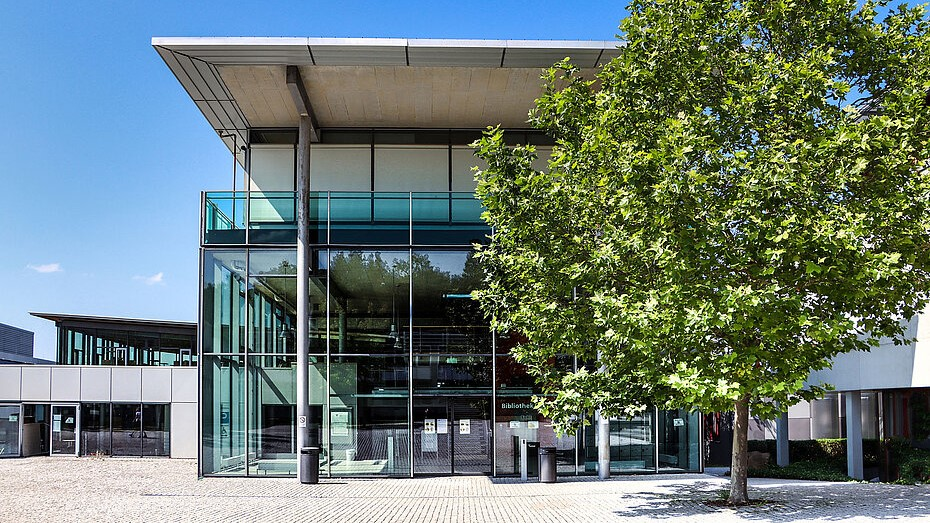
\includegraphics[width=\linewidth,height=\dimexpr\textheight\relax,keepaspectratio]{UiB-images/hspf.jpg}
\end{frame}

\begin{frame}{Deutsche Post DHL - Komissionierer}
  \centering
    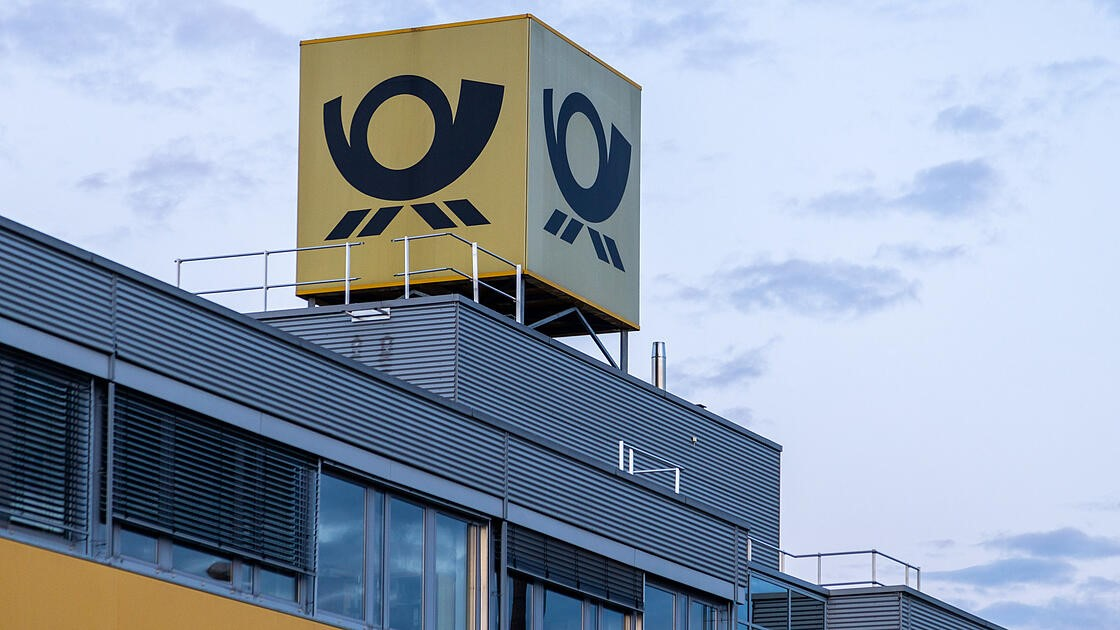
\includegraphics[width=\linewidth,height=\dimexpr\textheight\relax,keepaspectratio]{UiB-images/dpdhl.jpg}
\end{frame}

\begin{frame}{Lutz \& Grub Academy - Umschulung}
  \centering
    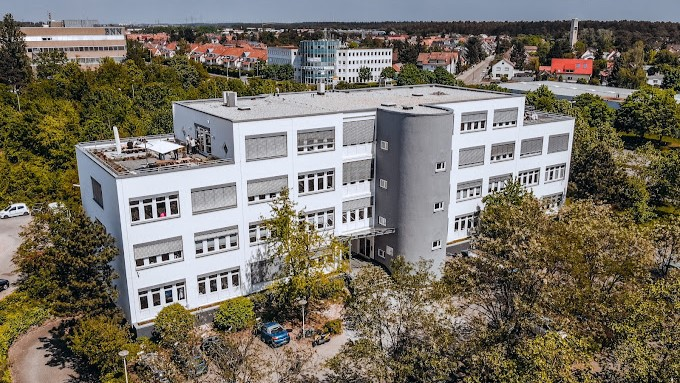
\includegraphics[width=\linewidth,height=\dimexpr\textheight\relax,keepaspectratio]{UiB-images/lug.jpg}
\end{frame}

\begin{frame}{pgx software solutions - Praxisphase}
  \centering
    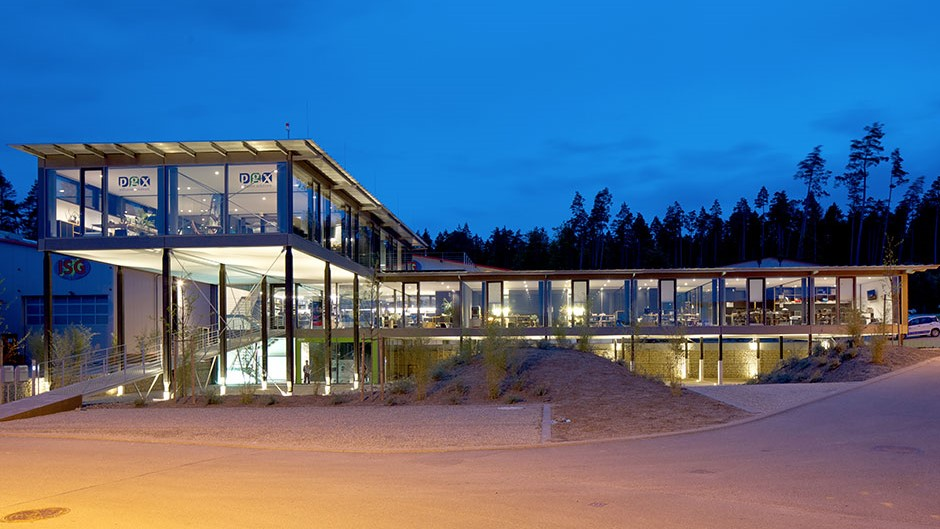
\includegraphics[width=\linewidth,height=\dimexpr\textheight\relax,keepaspectratio]{UiB-images/pgx.jpg}
\end{frame}

\begin{frame}{INIT - Software Developer}
  \centering
    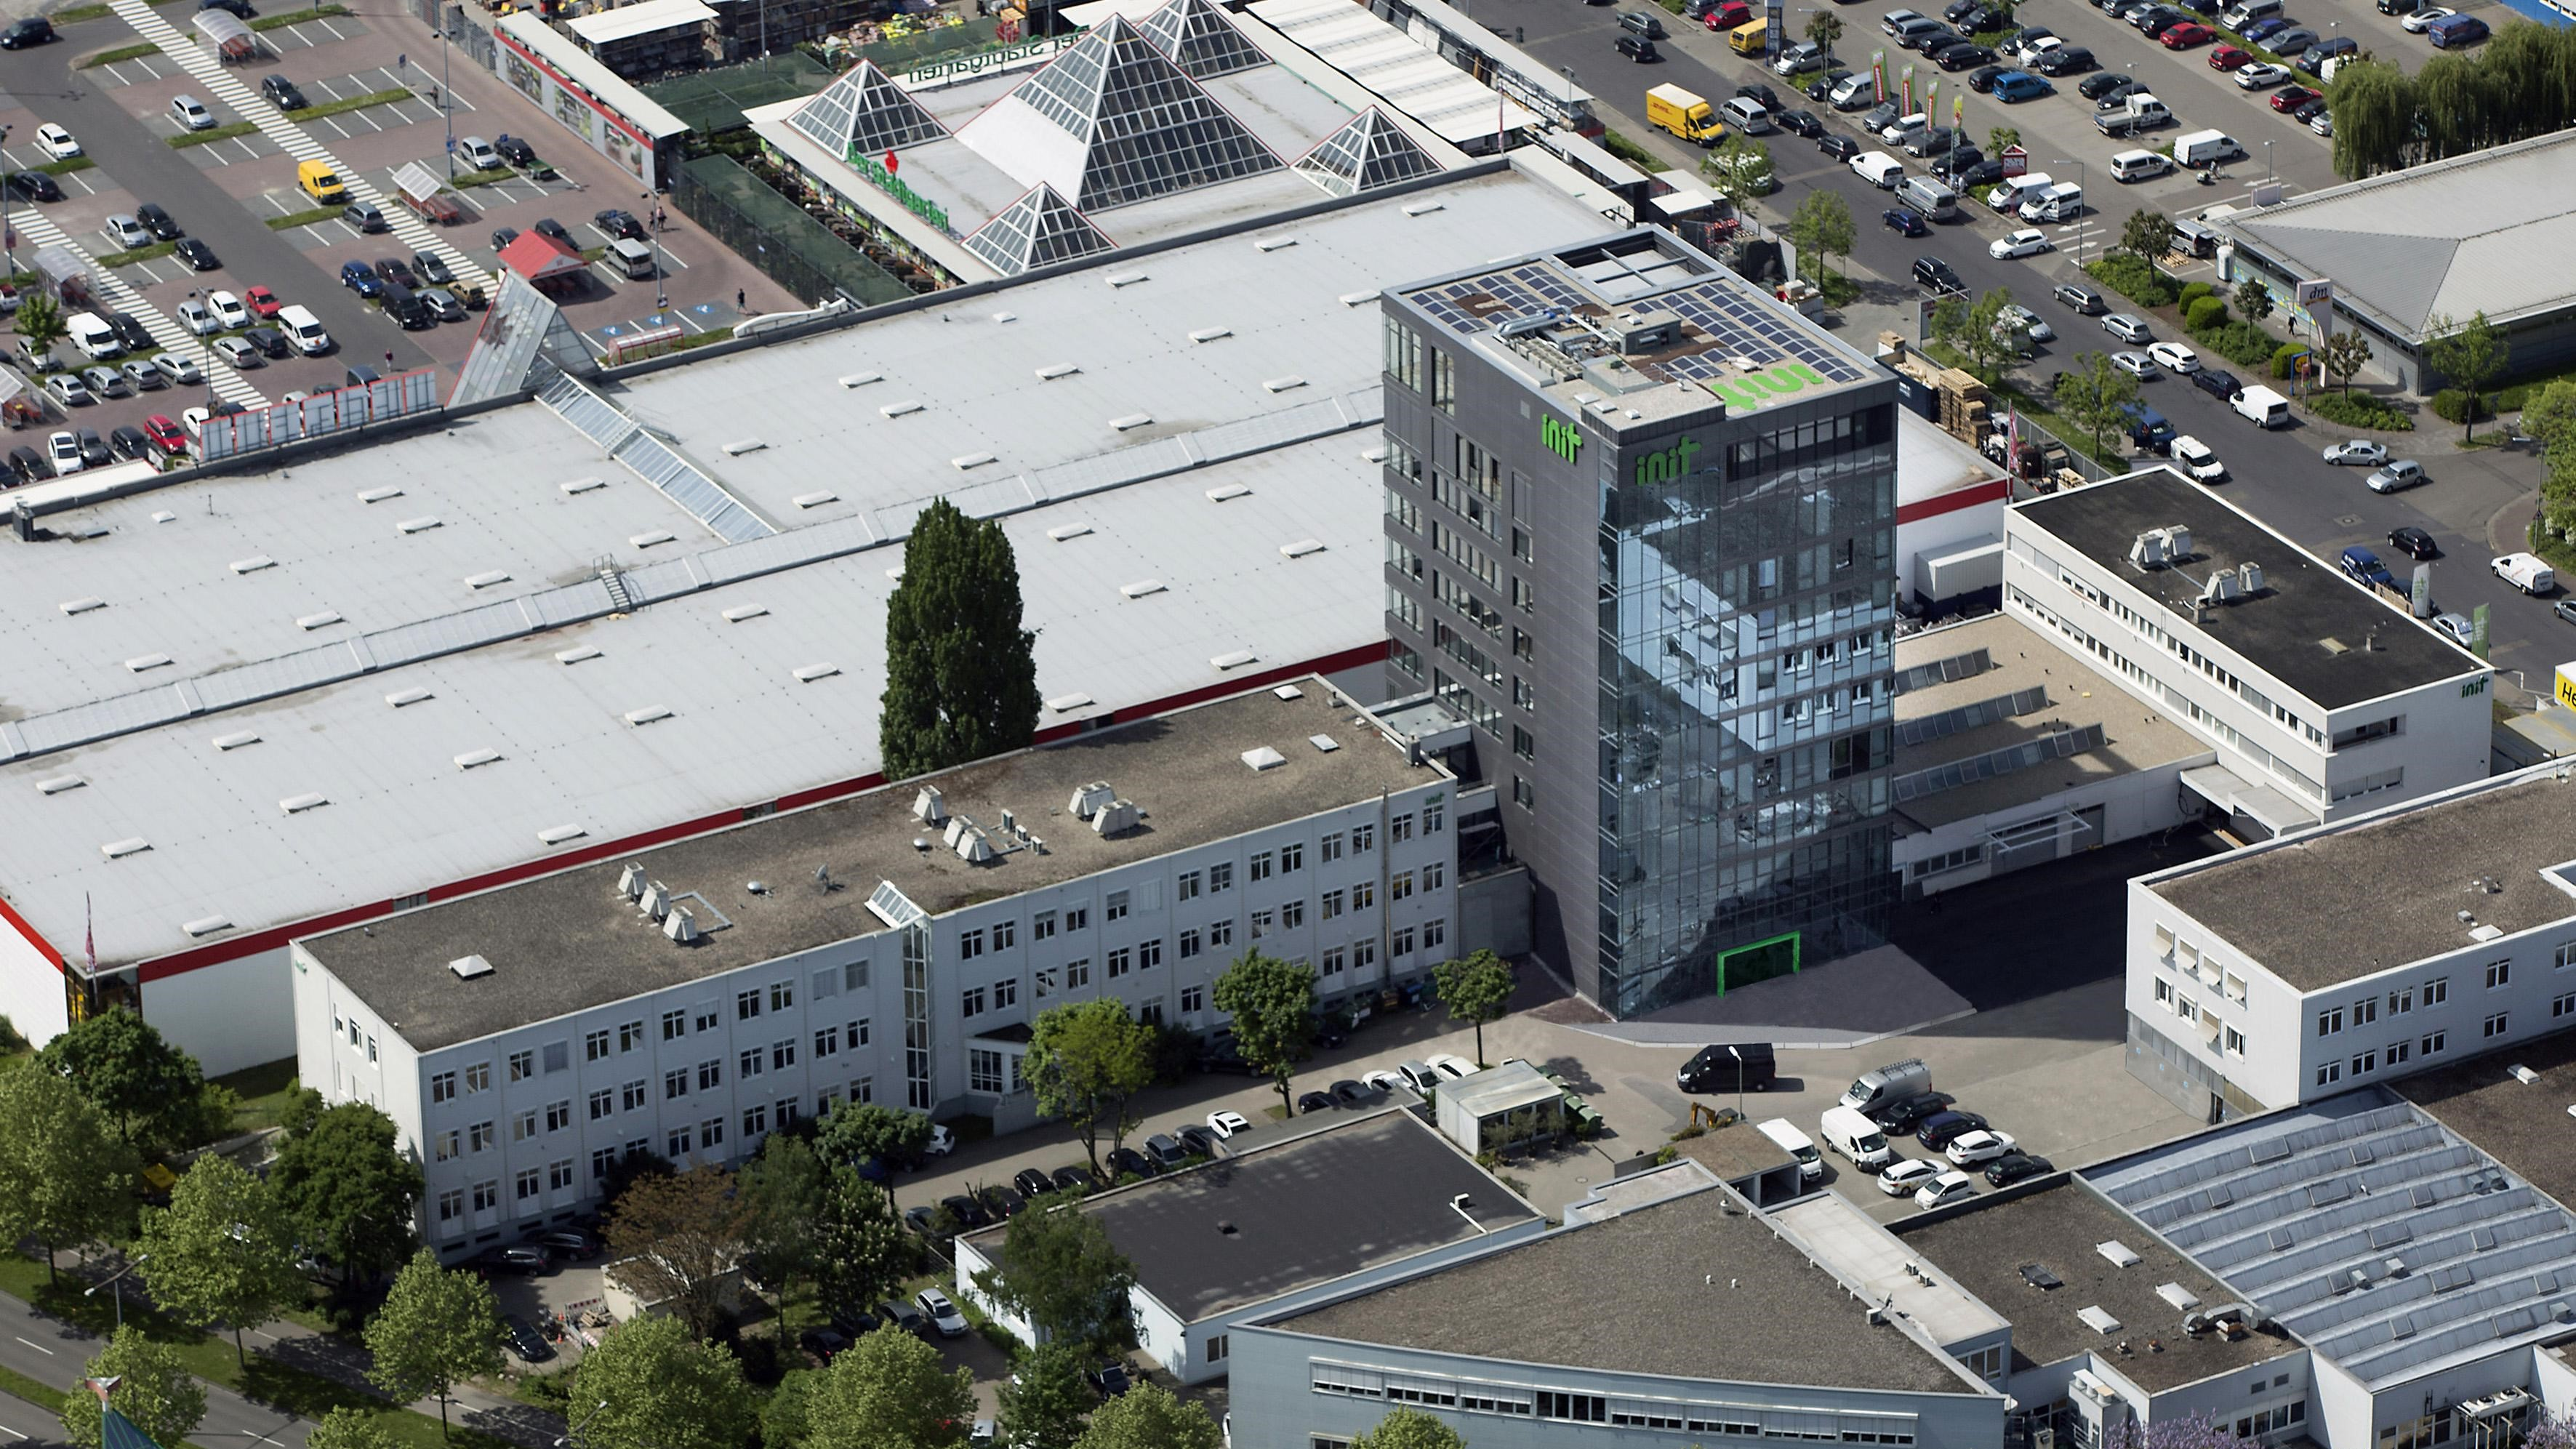
\includegraphics[width=\linewidth,height=\dimexpr\textheight\relax,keepaspectratio]{UiB-images/init.jpg}
\end{frame}
%%%%%%%%%%%%%%%%%%%%%%%%%%%%%%%%%%%%%%%%%%%%%%%%%%%%%%%%%%%%%%%%%% - KAP.1.2
% Kap.1 - Einführung - Zielgruppe - 1.2
\subsection{Zielgruppe}
\SubSectionPage
{
  \usebackgroundtemplate{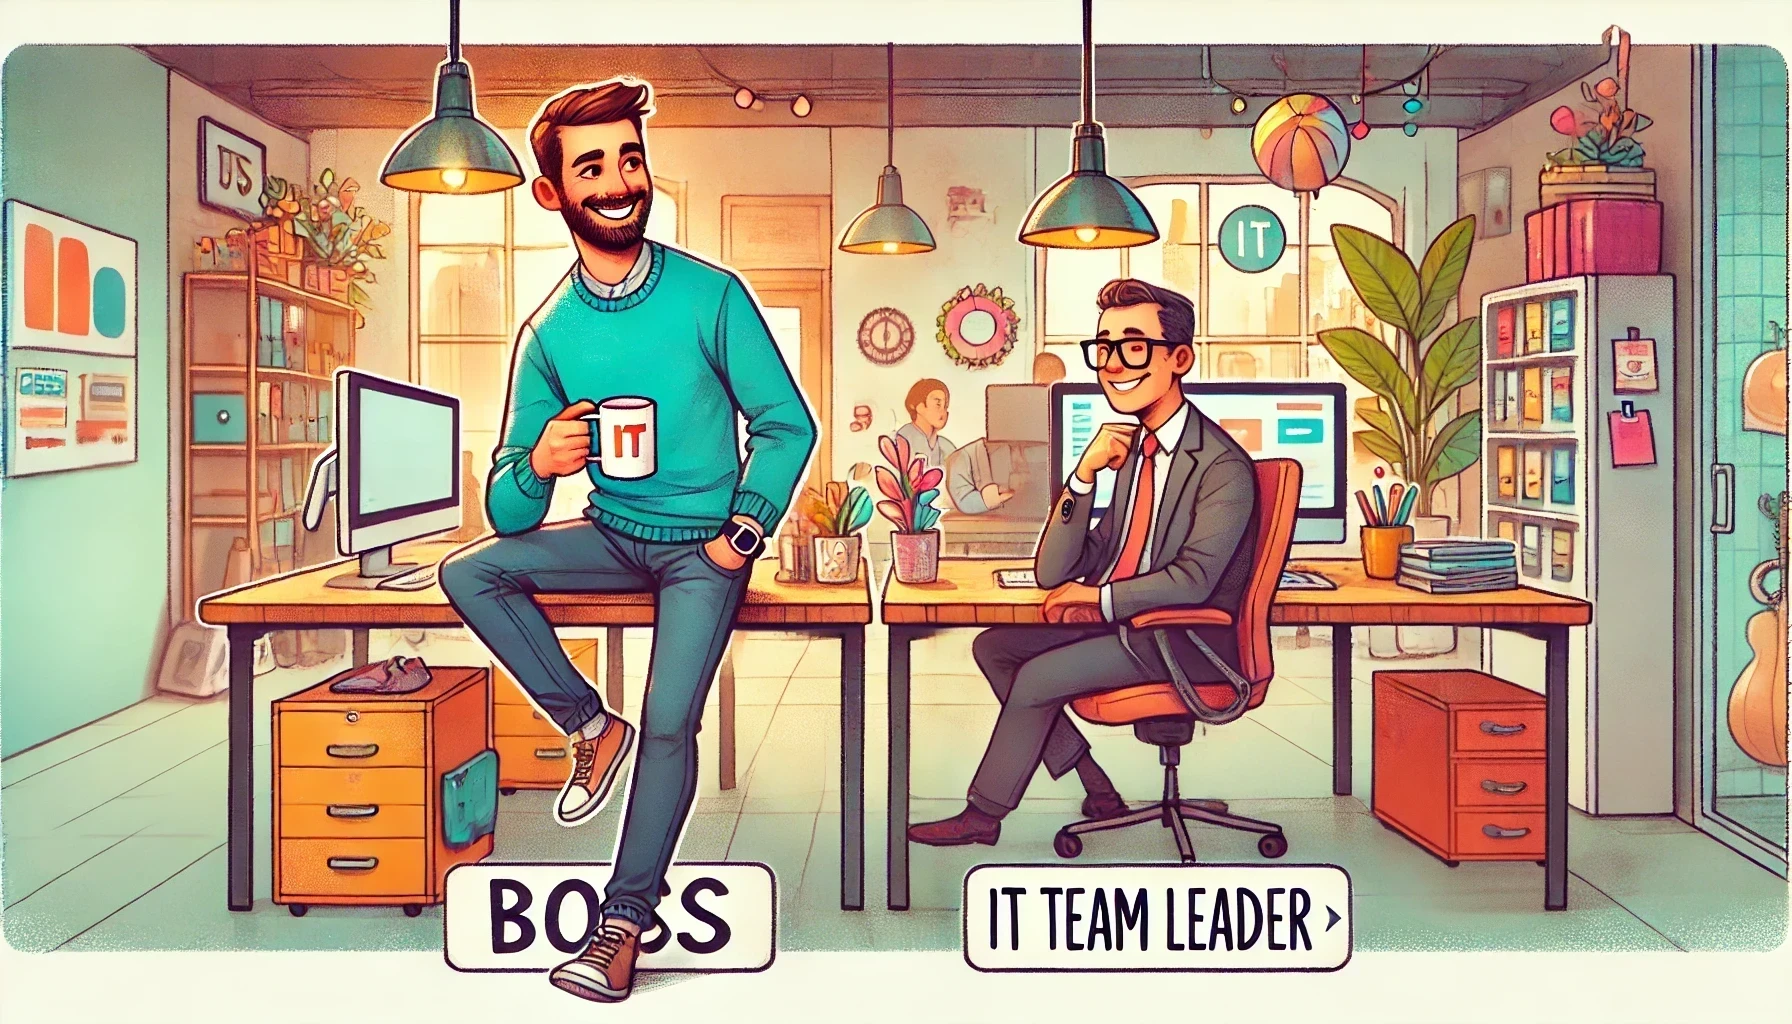
\includegraphics[width=\paperwidth,height=\paperheight]{UiB-images/zielgruppe_3.png}}
  \setbeamertemplate{navigation symbols}{}
  \begin{frame}[plain]
  \end{frame}
}
%%%%%%%%%%%%%%%%%%%%%%%%%%%%%%%%%%%%%%%%%%%%%%%%%%%%%%%%%%%%%%%%%%%% - KAP.2
% Kap.2 - Projektplanung und -umsetzung
\section{Projektplanung/-umsetzung}
\begin{frame}{Inhaltsverzeichnis}
  \vspace{3em}
  \hspace{1em}
  \begin{minipage}{0.48\textwidth}
    {\small
      \tableofcontents[sections={1-3}, currentsection]
    }
  \end{minipage}
  \hfill
  \begin{minipage}{0.48\textwidth}
    {\small
      \tableofcontents[sections={4-7}, currentsection]
    }
  \end{minipage}
\end{frame}
%%%%%%%%%%%%%%%%%%%%%%%%%%%%%%%%%%%%%%%%%%%%%%%%%%%%%%%%%%%%%%%%%% - KAP.2.1
% Kap.2 - Projektplanung und -umsetzung - Ausgangssituation - 2.1
\subsection{Ausgangssituation}
% \SubSectionPage
\foreach \x in {1,...,5} {
  \usebackgroundtemplate{\includegraphics[width=\paperwidth,height=\paperheight]{UiB-images/ausg/aus_\x.pdf}}
  \setbeamertemplate{navigation symbols}{}
  \begin{frame}[plain]
  \end{frame}
  \addtocounter{framenumber}{-1}
}
%%%%%%%%%%%%%%%%%%%%%%%%%%%%%%%%%%%%%%%%%%%%%%%%%%%%%%%%%%%%%%%%%% - KAP.2.2
% Kap.2 - Projektplanung und -umsetzung - Ist-Analyse - 2.2
\subsection{Ist-Analyse}
\addtocounter{framenumber}{+1}
\SubSectionPage
\foreach \x in {1,...,7} {
  \usebackgroundtemplate{\includegraphics[width=\paperwidth,height=\paperheight]{UiB-images/ist_analyse/ist_\x.pdf}}
  \setbeamertemplate{navigation symbols}{}
  \begin{frame}[plain]
  \end{frame}
  \addtocounter{framenumber}{-1}
}
%%%%%%%%%%%%%%%%%%%%%%%%%%%%%%%%%%%%%%%%%%%%%%%%%%%%%%%%%%%%%%%%%% - KAP.2.3
% Kap.2 - Projektplanung und -umsetzung - Soll-Konzept - 2.3
\subsection{Soll-Konzept}
\addtocounter{framenumber}{+1}
\SubSectionPage
\foreach \x in {1,...,12} {
  \usebackgroundtemplate{\includegraphics[width=\paperwidth,height=\paperheight]{UiB-images/soll_konzept/soll_\x.pdf}}
  \setbeamertemplate{navigation symbols}{}
  \begin{frame}[plain]
  \end{frame}
  \addtocounter{framenumber}{-1}
}
%%%%%%%%%%%%%%%%%%%%%%%%%%%%%%%%%%%%%%%%%%%%%%%%%%%%%%%%%%%%%%%%%% - EXCLUDE
% Kap.2 - Projektplanung und -umsetzung - Soll-Ist-Vergleich - 2.4
% \subsection{Soll-Ist-Vergleich}
% \SubSectionPage
% \begin{frame}{Soll-Ist-Vergleich}\pause
%   \begin{block}{Ergebnisse}\pause
%     \begin{itemize}
%       \item \textbf{Alle Aufgaben wurden erfolgreich abgeschlossen.}
%     \end{itemize}
%   \end{block}\pause
%   \begin{block}{Abweichungen}\pause
%     \begin{itemize}
%       \item \textbf{E-Mail-Service}\pause
%       \begin{itemize}
%         \item \textbf{Flexible E-Mail-Klassen statt vollständiger E-Mail-Logik.}\pause
%         \item \textbf{HTML-Vorlagen.}
%       \end{itemize}
%     \end{itemize}
%   \end{block}\pause
%   \begin{block}{Herausforderungen}\pause
%     \begin{itemize}
%       \item \textbf{Mehrsprachigkeit}\pause
%       \begin{itemize}
%         \item \textbf{Einführung von Deutsch- und Englisch-Ressourcen.}\pause
%         \item \textbf{Übersetzung durch Zeitersparnis beim Dashboard problemlos umgesetzt.}
%       \end{itemize}
%     \end{itemize}
%   \end{block}
% \end{frame}
%%%%%%%%%%%%%%%%%%%%%%%%%%%%%%%%%%%%%%%%%%%%%%%%%%%%%%%%%%%%%%%%%%%% - KAP.3
% Kap.3 - Wirtschaftlichkeit
\section{Wirtschaftlichkeit}
\addtocounter{framenumber}{+1}
\begin{frame}{Inhaltsverzeichnis}
  \vspace{3em}
  \hspace{1em}
  \begin{minipage}{0.48\textwidth}
    {\small
      \tableofcontents[sections={1-3}, currentsection]
    }
  \end{minipage}
  \hfill
  \begin{minipage}{0.48\textwidth}
    {\small
      \tableofcontents[sections={4-7}, currentsection]
    }
  \end{minipage}
\end{frame}
% \SectionPage
%%%%%%%%%%%%%%%%%%%%%%%%%%%%%%%%%%%%%%%%%%%%%%%%%%%%%%%%%%%%%%%%%% - KAP.3.1
% Kap.3 - Wirtschaftlichkeit - GK - 3.1
\subsection{Gesamtkosten}
% \SubSectionPage
\foreach \x in {1,...,4} {
  \usebackgroundtemplate{\includegraphics[width=\paperwidth,height=\paperheight]{UiB-images/gk/gk_\x.pdf}}
  \setbeamertemplate{navigation symbols}{}
  \begin{frame}[plain]
  \end{frame}
  \addtocounter{framenumber}{-1}
}
%%%%%%%%%%%%%%%%%%%%%%%%%%%%%%%%%%%%%%%%%%%%%%%%%%%%%%%%%%%%%%%%%% - KAP.3.2
% Kap.3 - Wirtschaftlichkeit - Amo - 3.2
\subsection{Amortisation}
\addtocounter{framenumber}{+1}
% \SubSectionPage
\foreach \x in {1,...,4} {
  \usebackgroundtemplate{\includegraphics[width=\paperwidth,height=\paperheight]{UiB-images/amo/amo_\x.pdf}}
  \setbeamertemplate{navigation symbols}{}
  \begin{frame}[plain]
  \end{frame}
  \addtocounter{framenumber}{-1}
}
%%%%%%%%%%%%%%%%%%%%%%%%%%%%%%%%%%%%%%%%%%%%%%%%%%%%%%%%%%%%%%%%%%%% - KAP.4
% Kap.4 - Design
\section{Design}
\addtocounter{framenumber}{+1}
\begin{frame}{Inhaltsverzeichnis}
  \vspace{3em}
  \hspace{1em}
  \begin{minipage}{0.48\textwidth}
    {\small
      \tableofcontents[sections={1-3}, currentsection]
    }
  \end{minipage}
  \hfill
  \begin{minipage}{0.48\textwidth}
    {\small
      \tableofcontents[sections={4-7}, currentsection]
    }
  \end{minipage}
\end{frame}
%\SectionPage
%%%%%%%%%%%%%%%%%%%%%%%%%%%%%%%%%%%%%%%%%%%%%%%%%%%%%%%%%%%%%%%%%% - KAP.4.1
% Kap.4 - Design - Registrierung und Login - 4.1
\subsection{Login}
% \SubSectionPage
{
  \usebackgroundtemplate{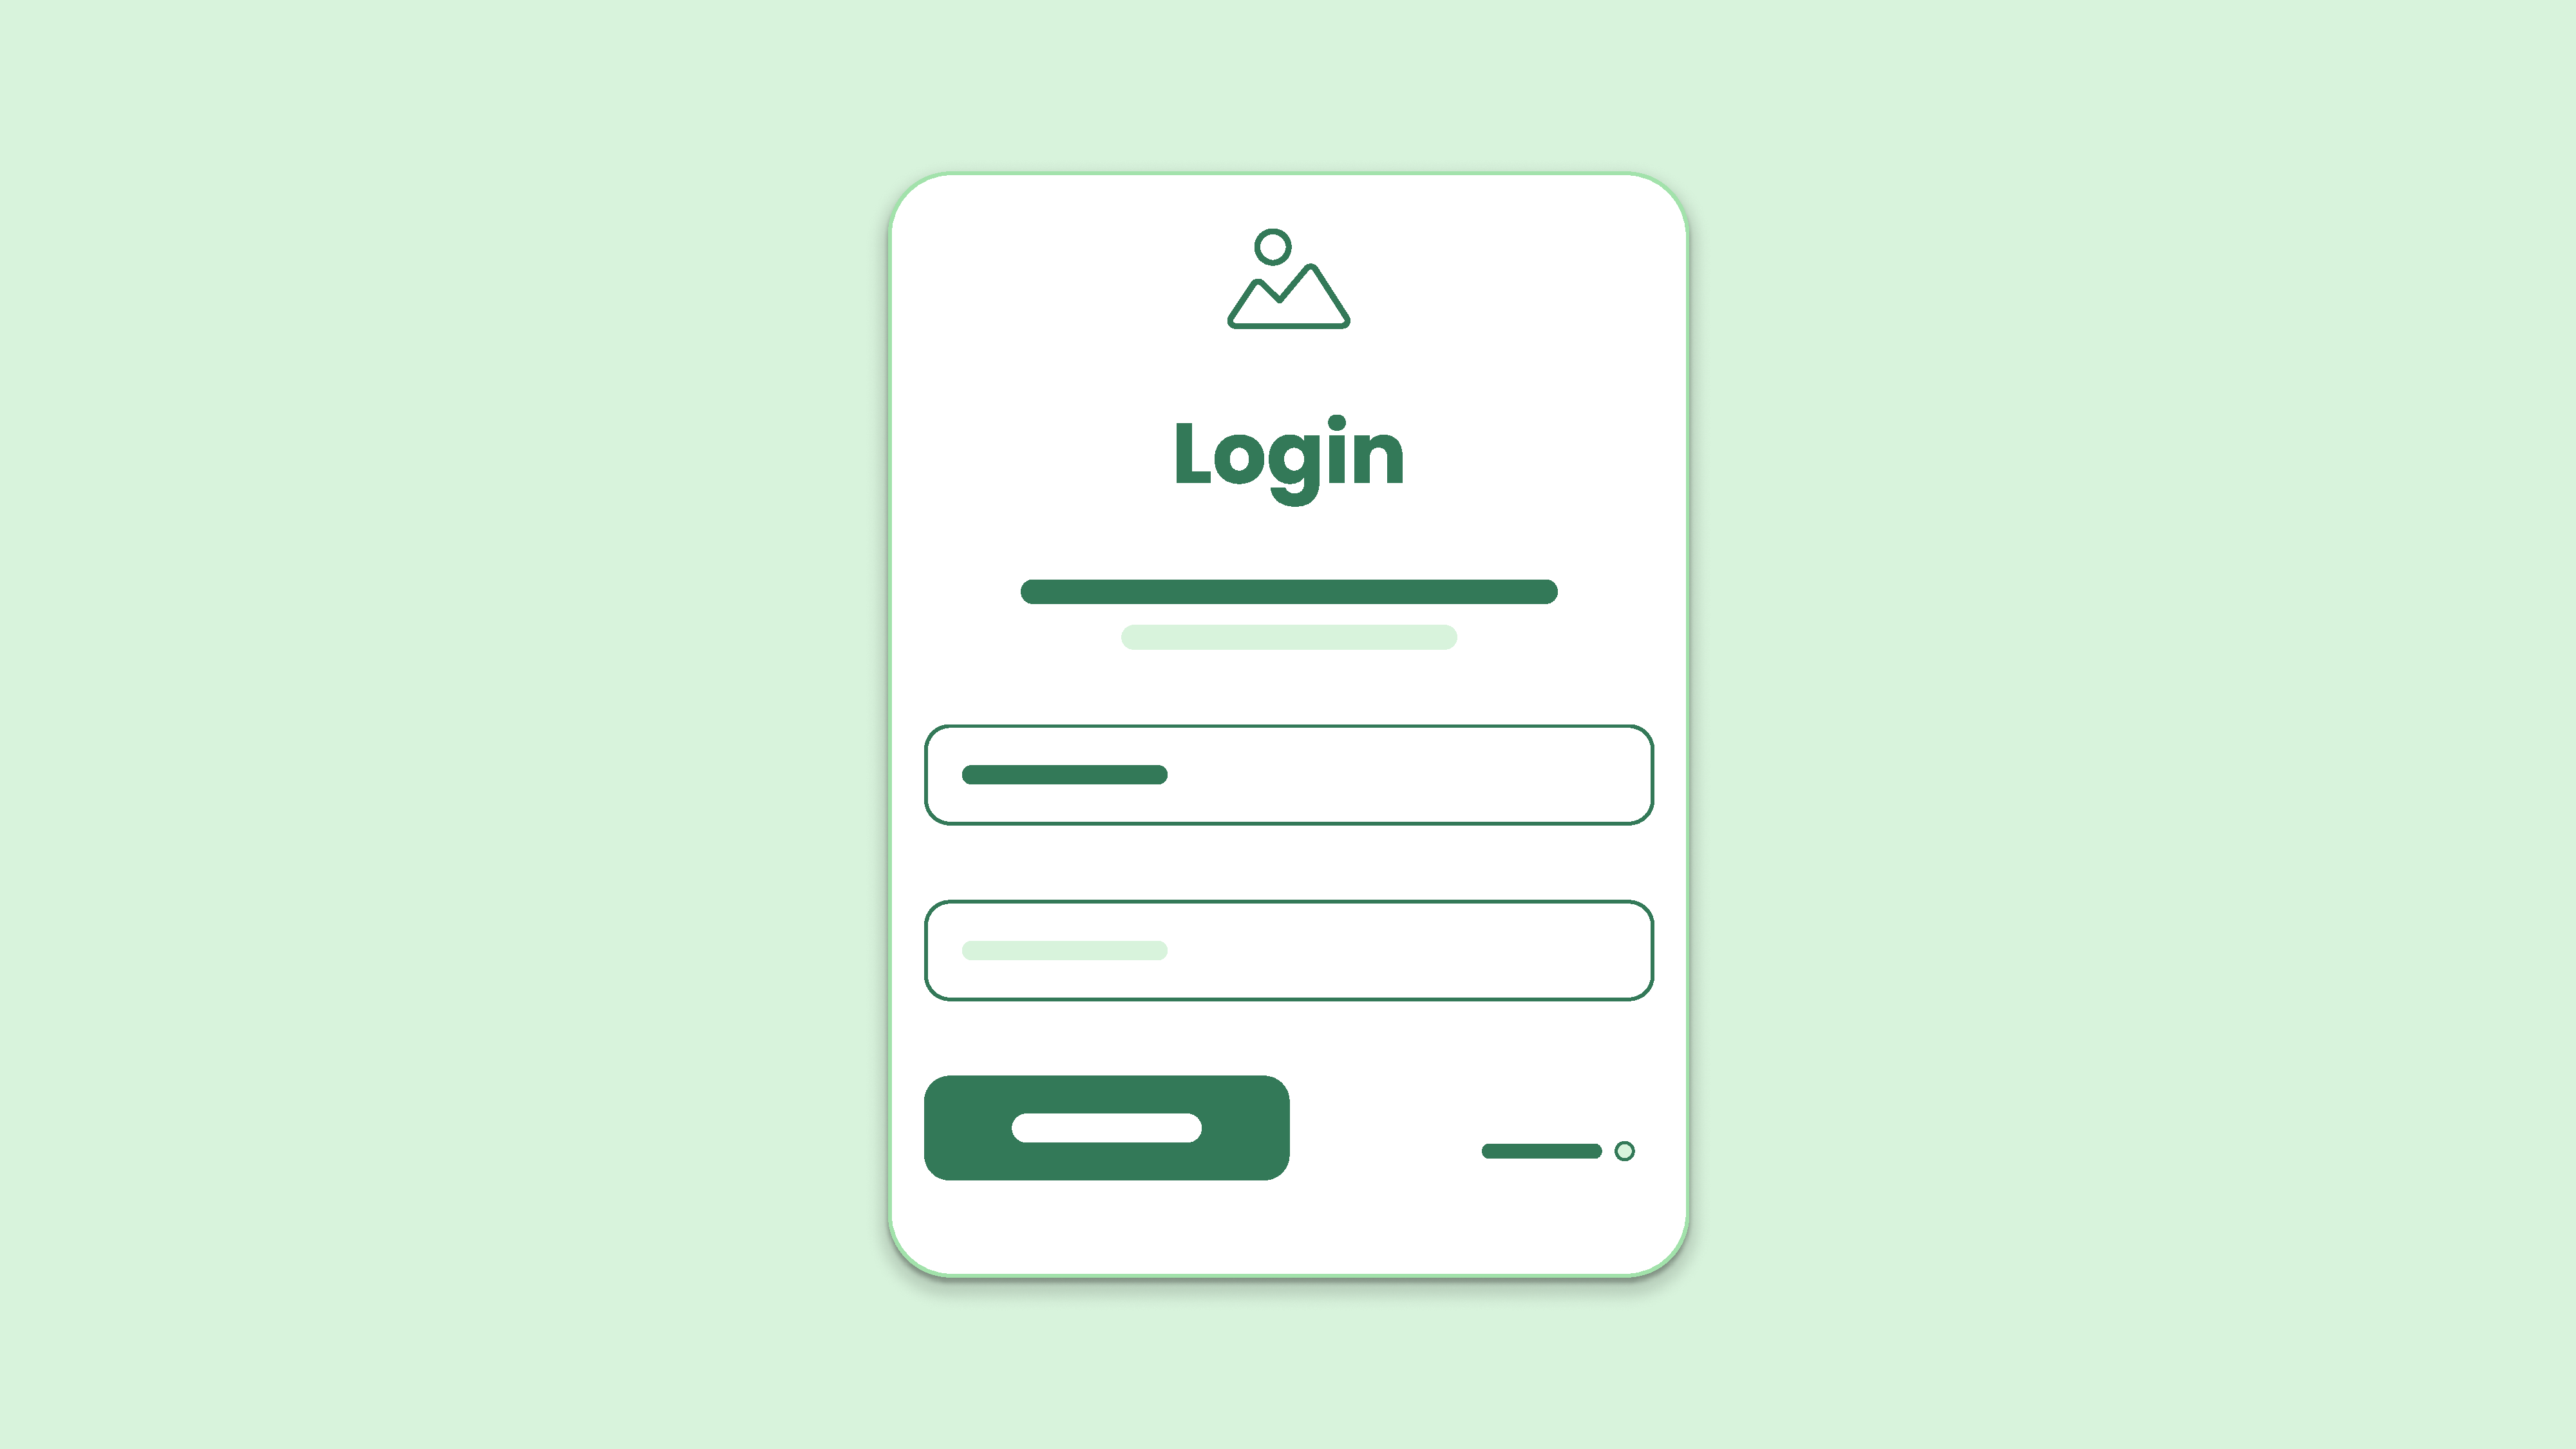
\includegraphics[width=\paperwidth,height=\paperheight]{UiB-images/mockups/Login - V1.pdf}}
  \setbeamertemplate{navigation symbols}{}
  \begin{frame}[plain]
  \end{frame}
  \addtocounter{framenumber}{-1}
}
{
  \usebackgroundtemplate{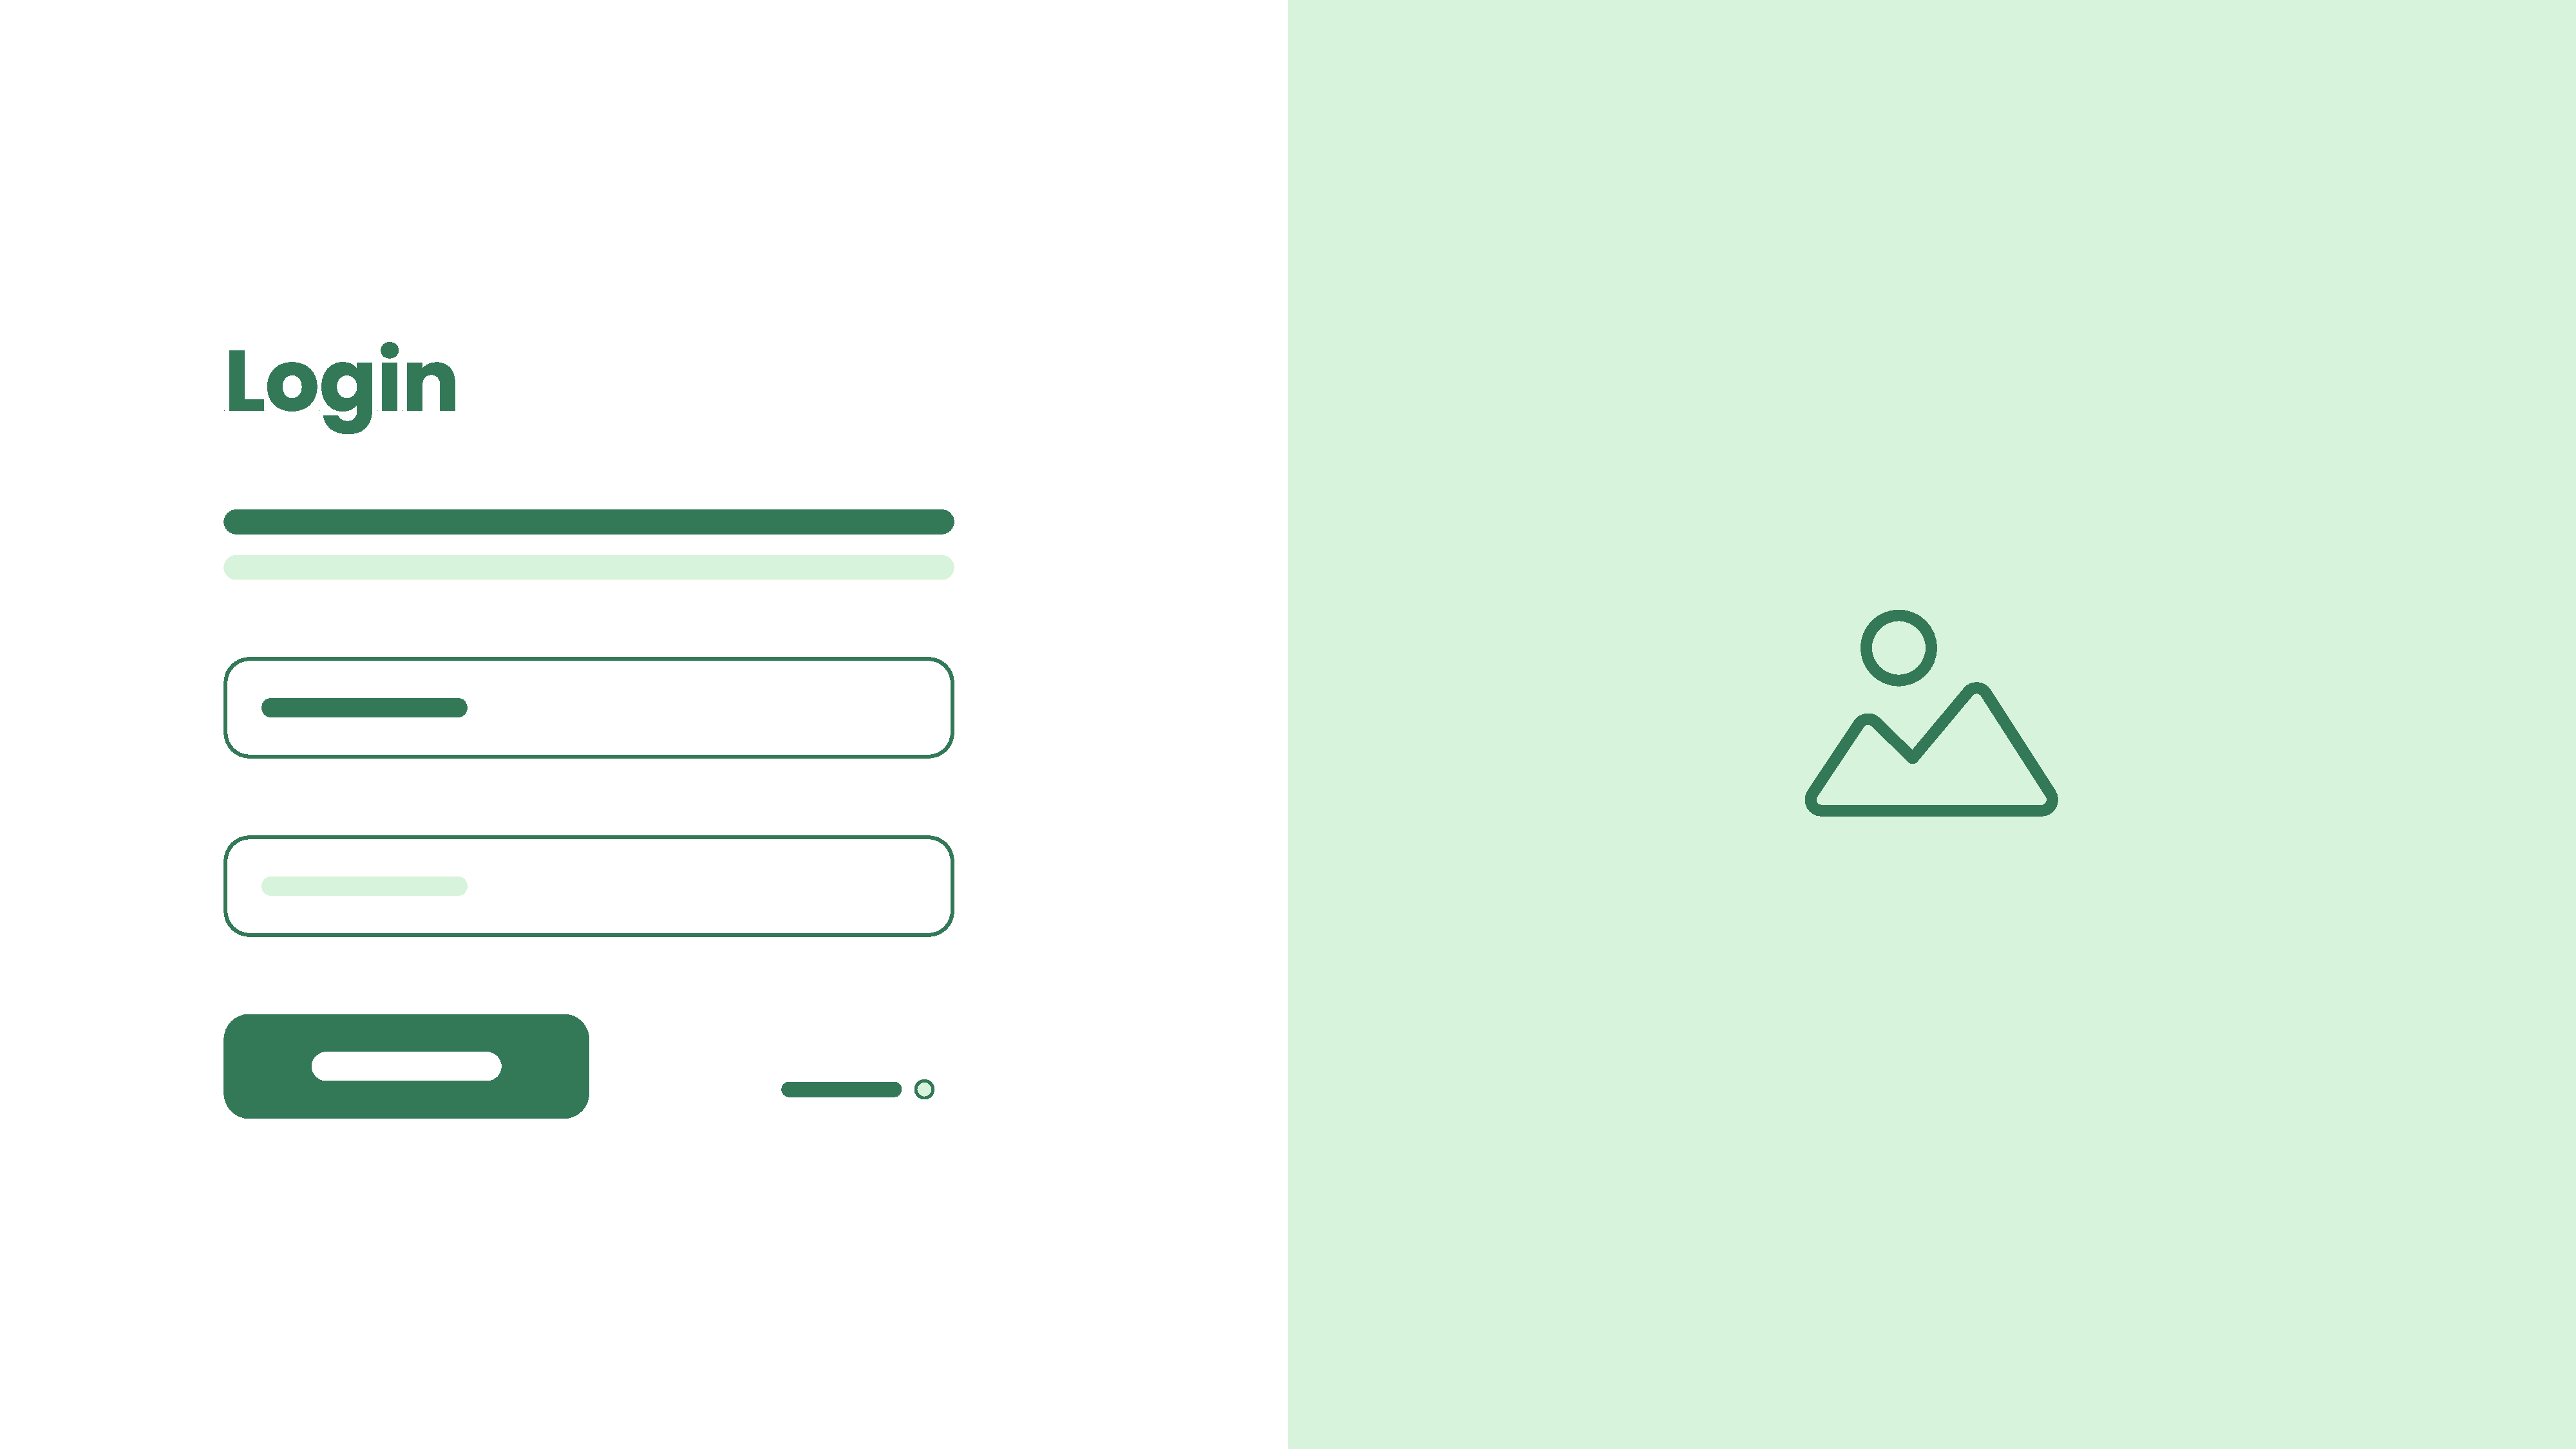
\includegraphics[width=\paperwidth,height=\paperheight]{UiB-images/mockups/Login - V2.pdf}}
  \setbeamertemplate{navigation symbols}{}
  \begin{frame}[plain]
  \end{frame}
  \addtocounter{framenumber}{-1}
}
{
  \usebackgroundtemplate{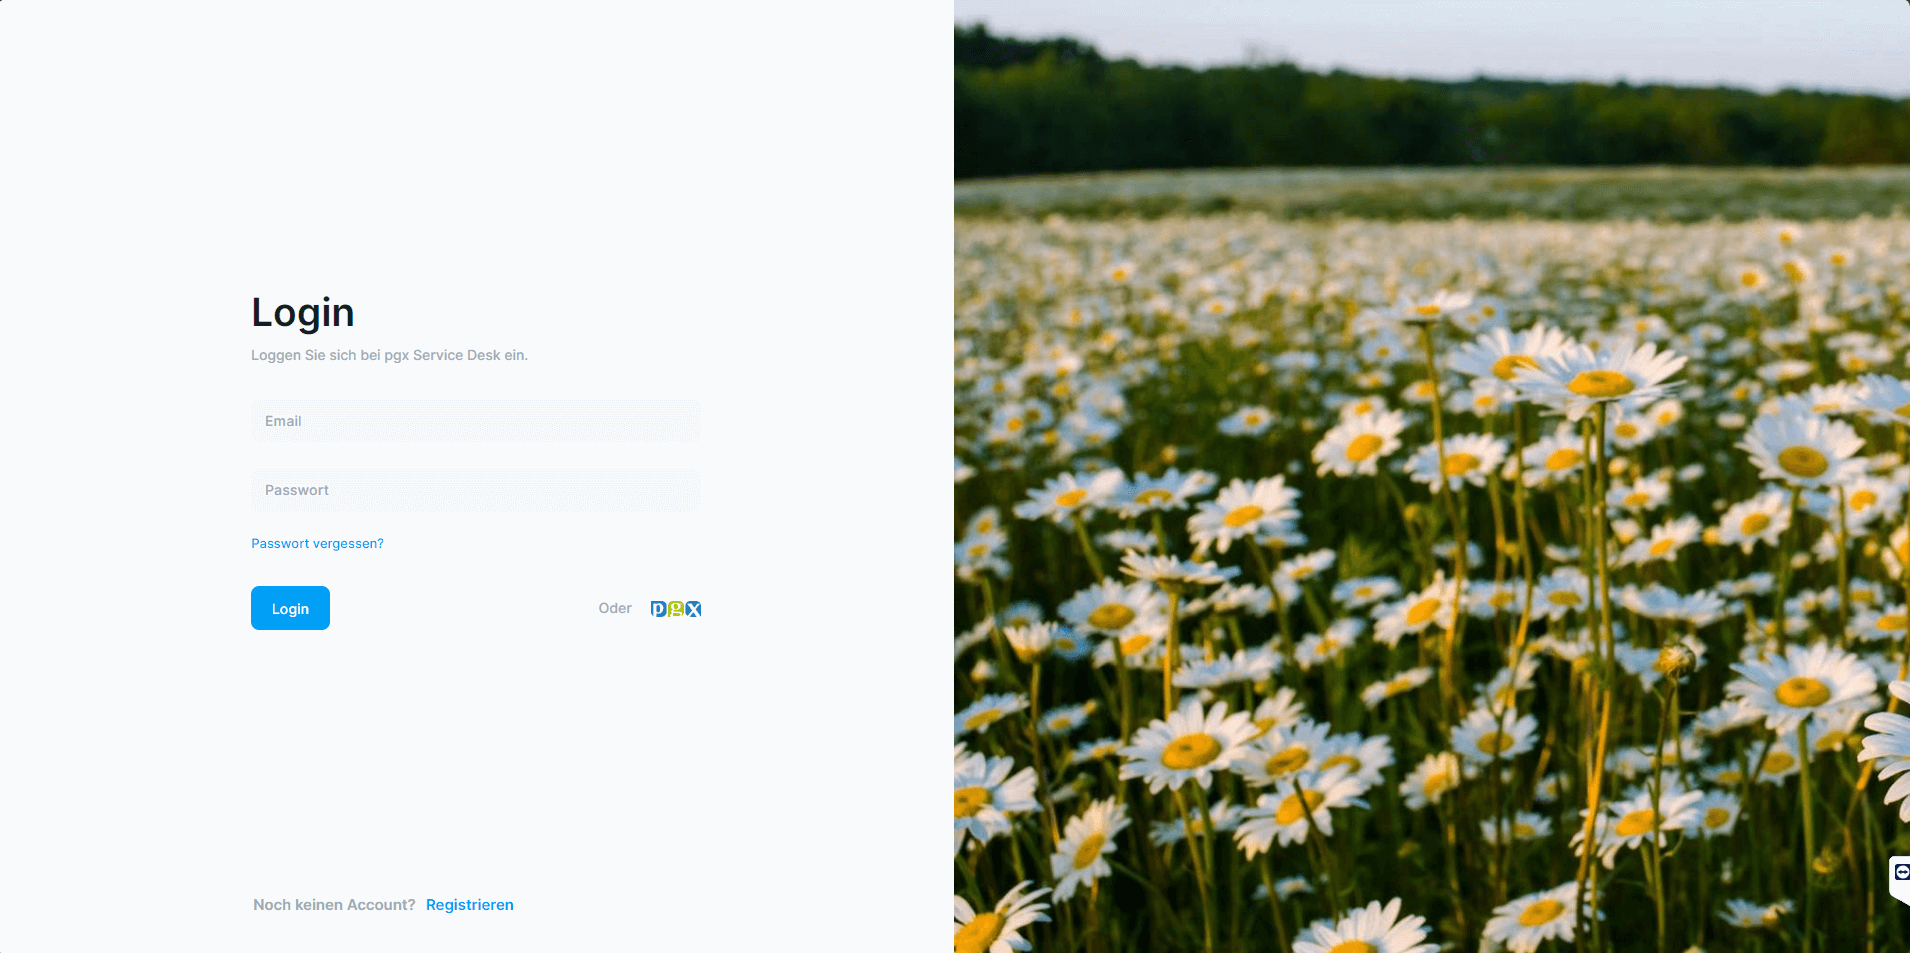
\includegraphics[width=\paperwidth,height=\paperheight]{UiB-images/mockups/login_cropped.png}}
  \setbeamertemplate{navigation symbols}{}
  \begin{frame}[plain]
  \end{frame}
  \addtocounter{framenumber}{-1}
}
{
  \usebackgroundtemplate{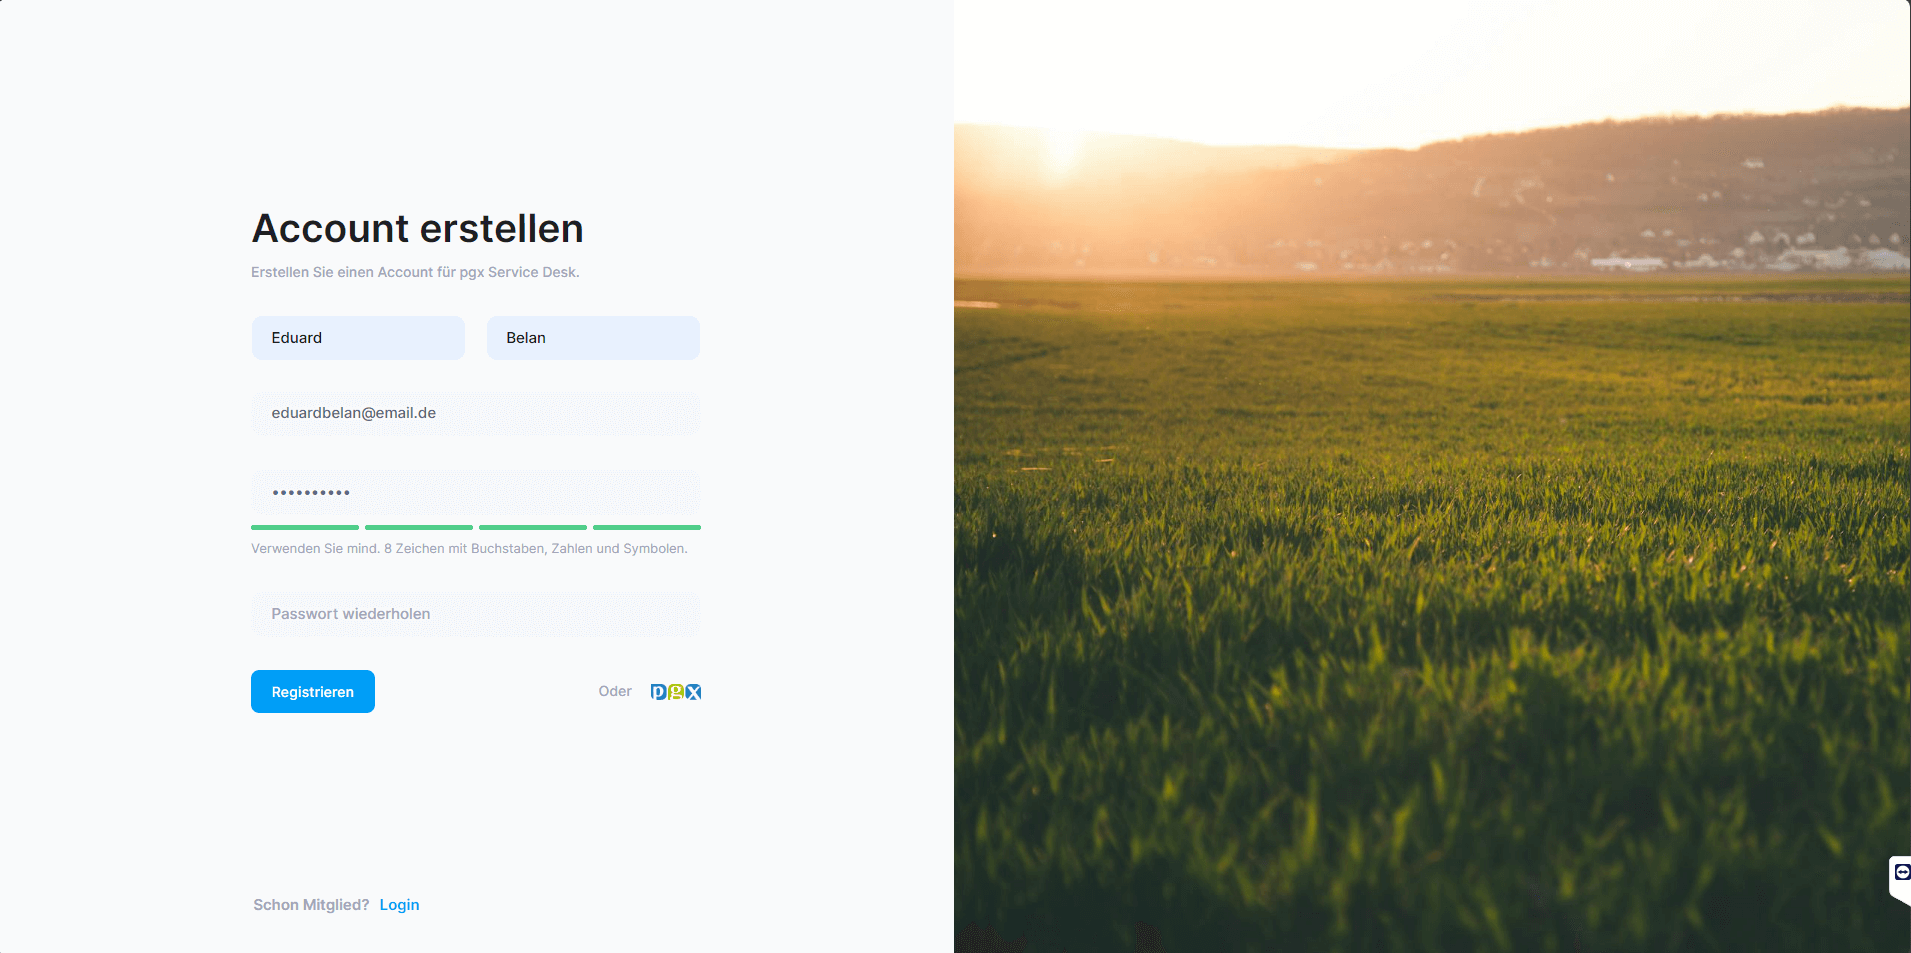
\includegraphics[width=\paperwidth,height=\paperheight]{UiB-images/mockups/registrieren_cropped.png}}
  \setbeamertemplate{navigation symbols}{}
  \begin{frame}[plain]
  \end{frame}
}
%%%%%%%%%%%%%%%%%%%%%%%%%%%%%%%%%%%%%%%%%%%%%%%%%%%%%%%%%%%%%%%%%% - KAP.4.2
% Kap.4 - Design - Dashboard - 4.2
\subsection{Dashboard}
\SubSectionPage
{
  \usebackgroundtemplate{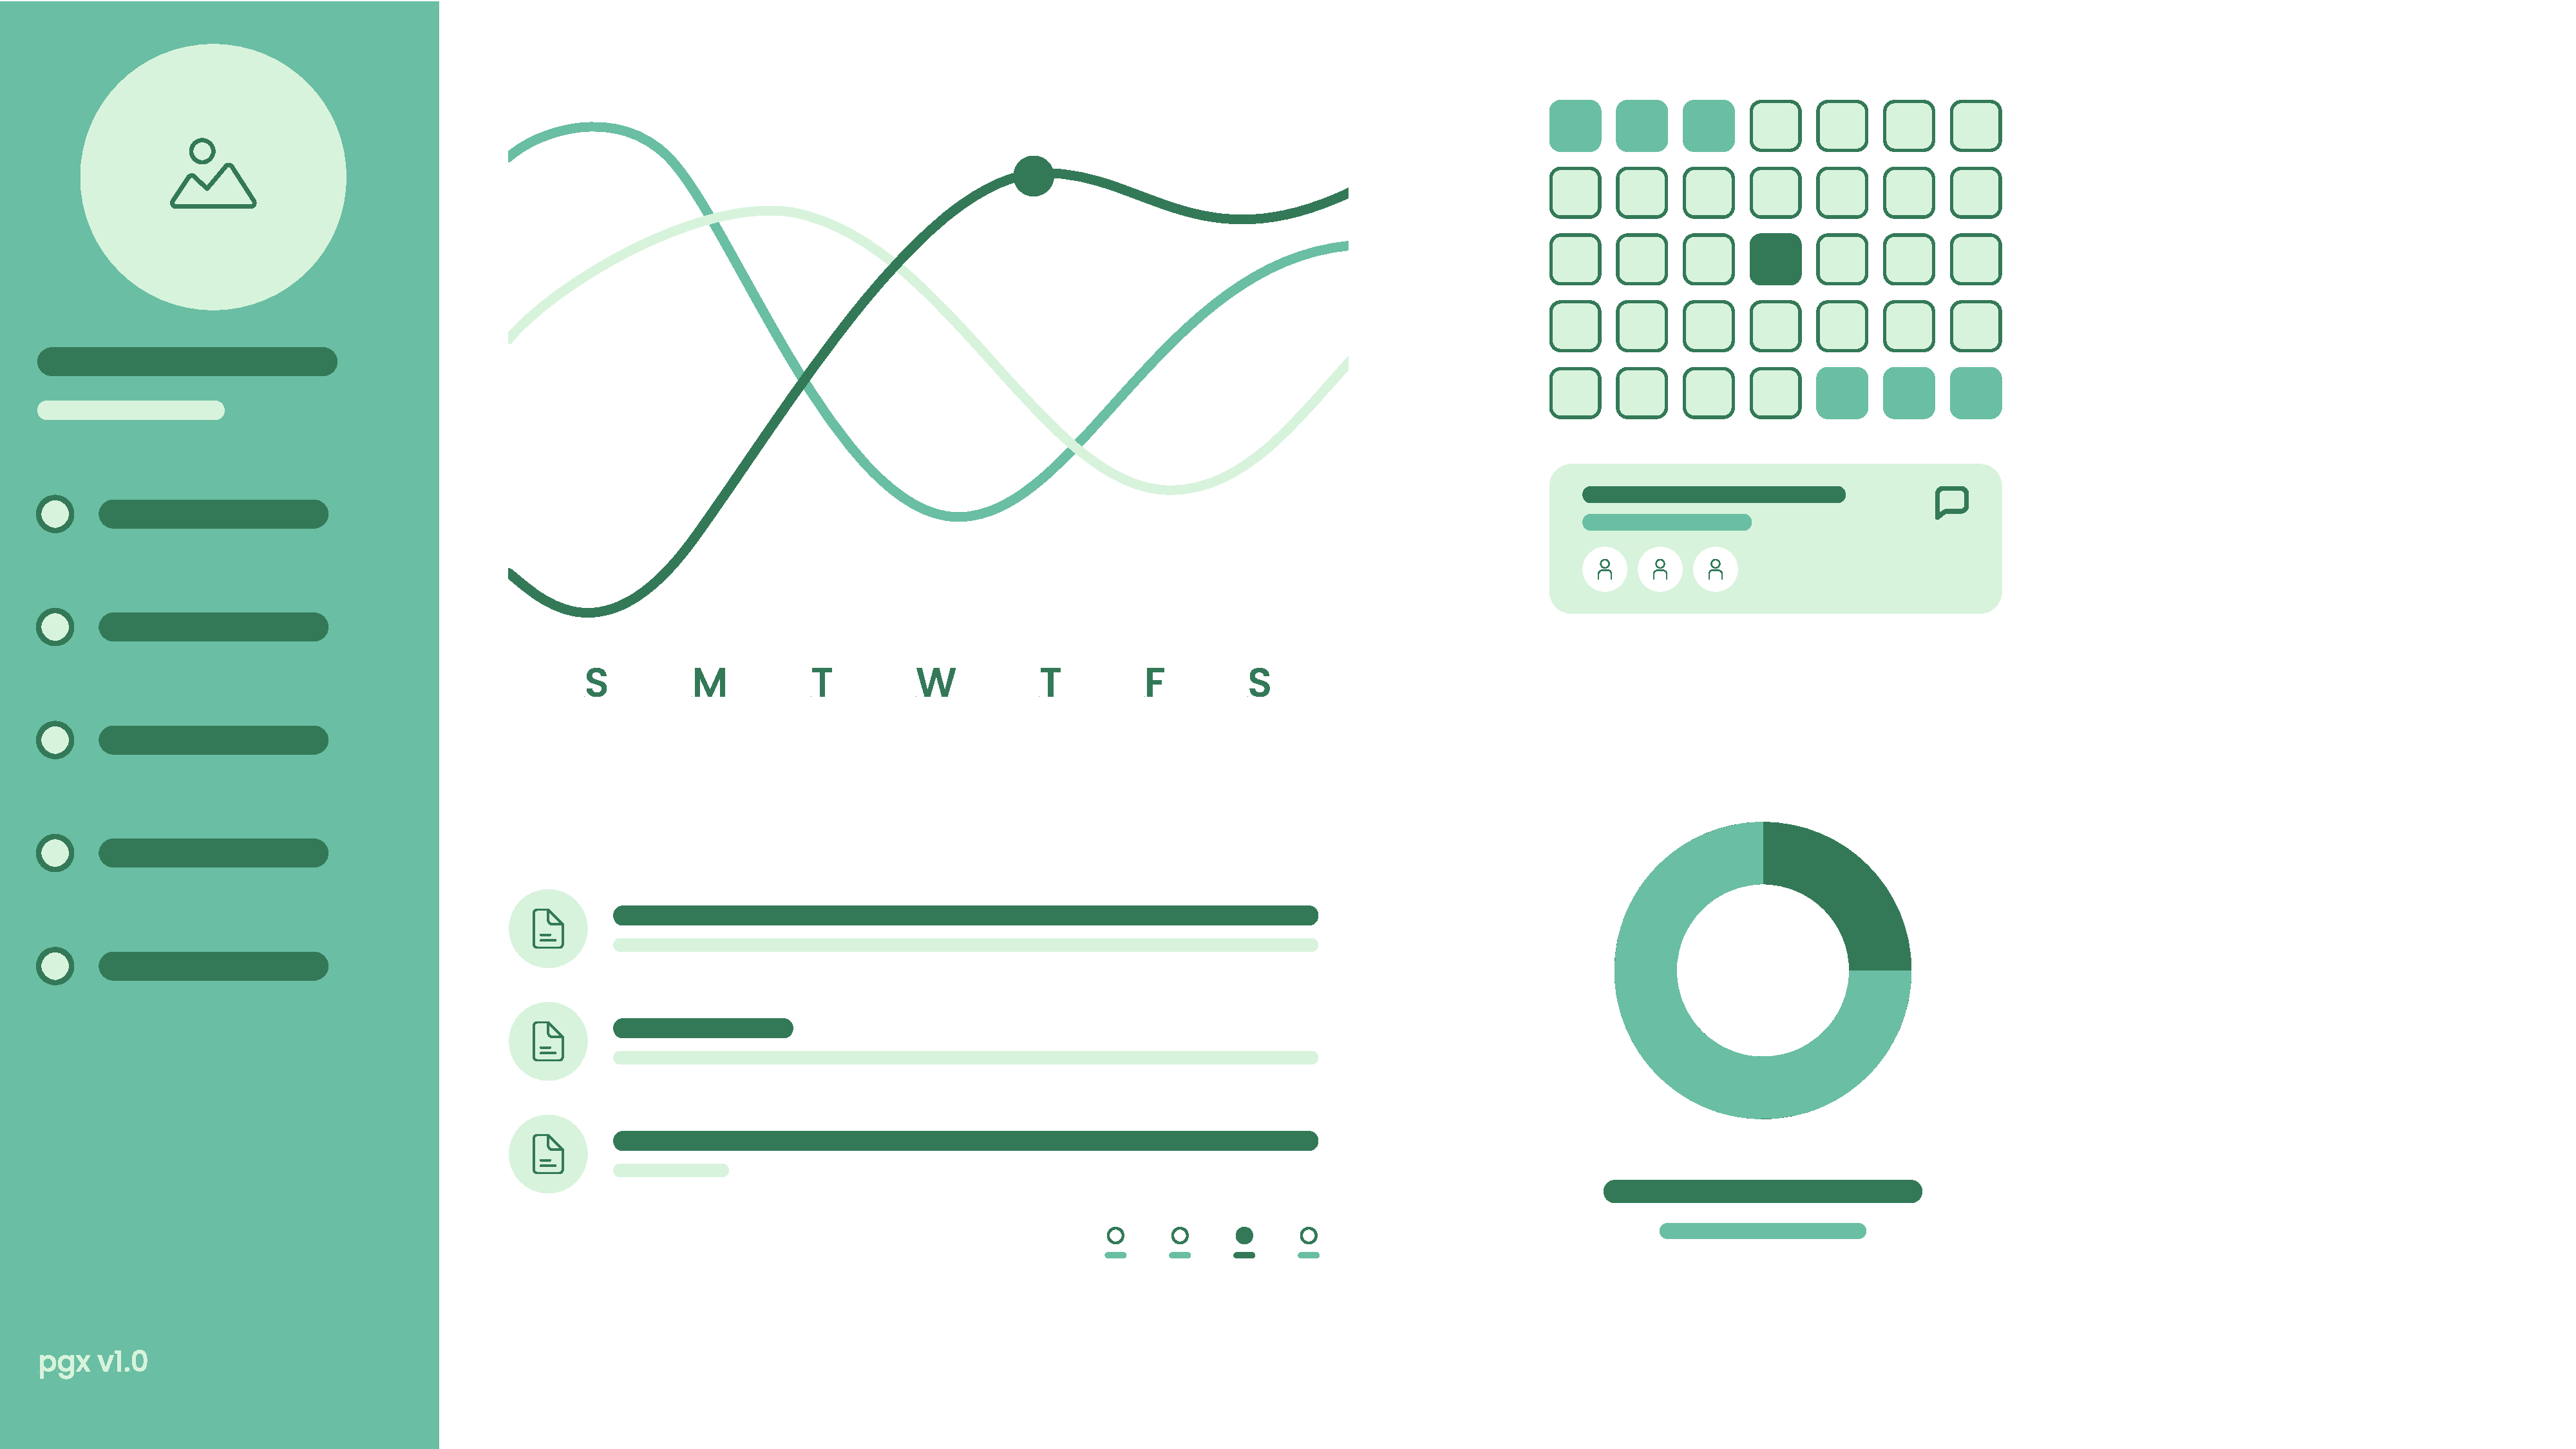
\includegraphics[width=\paperwidth,height=\paperheight]{UiB-images/mockups/Dashboard.pdf}}
  \setbeamertemplate{navigation symbols}{}
  \begin{frame}[plain]
  \end{frame}
  \addtocounter{framenumber}{-1}
}
{
  \usebackgroundtemplate{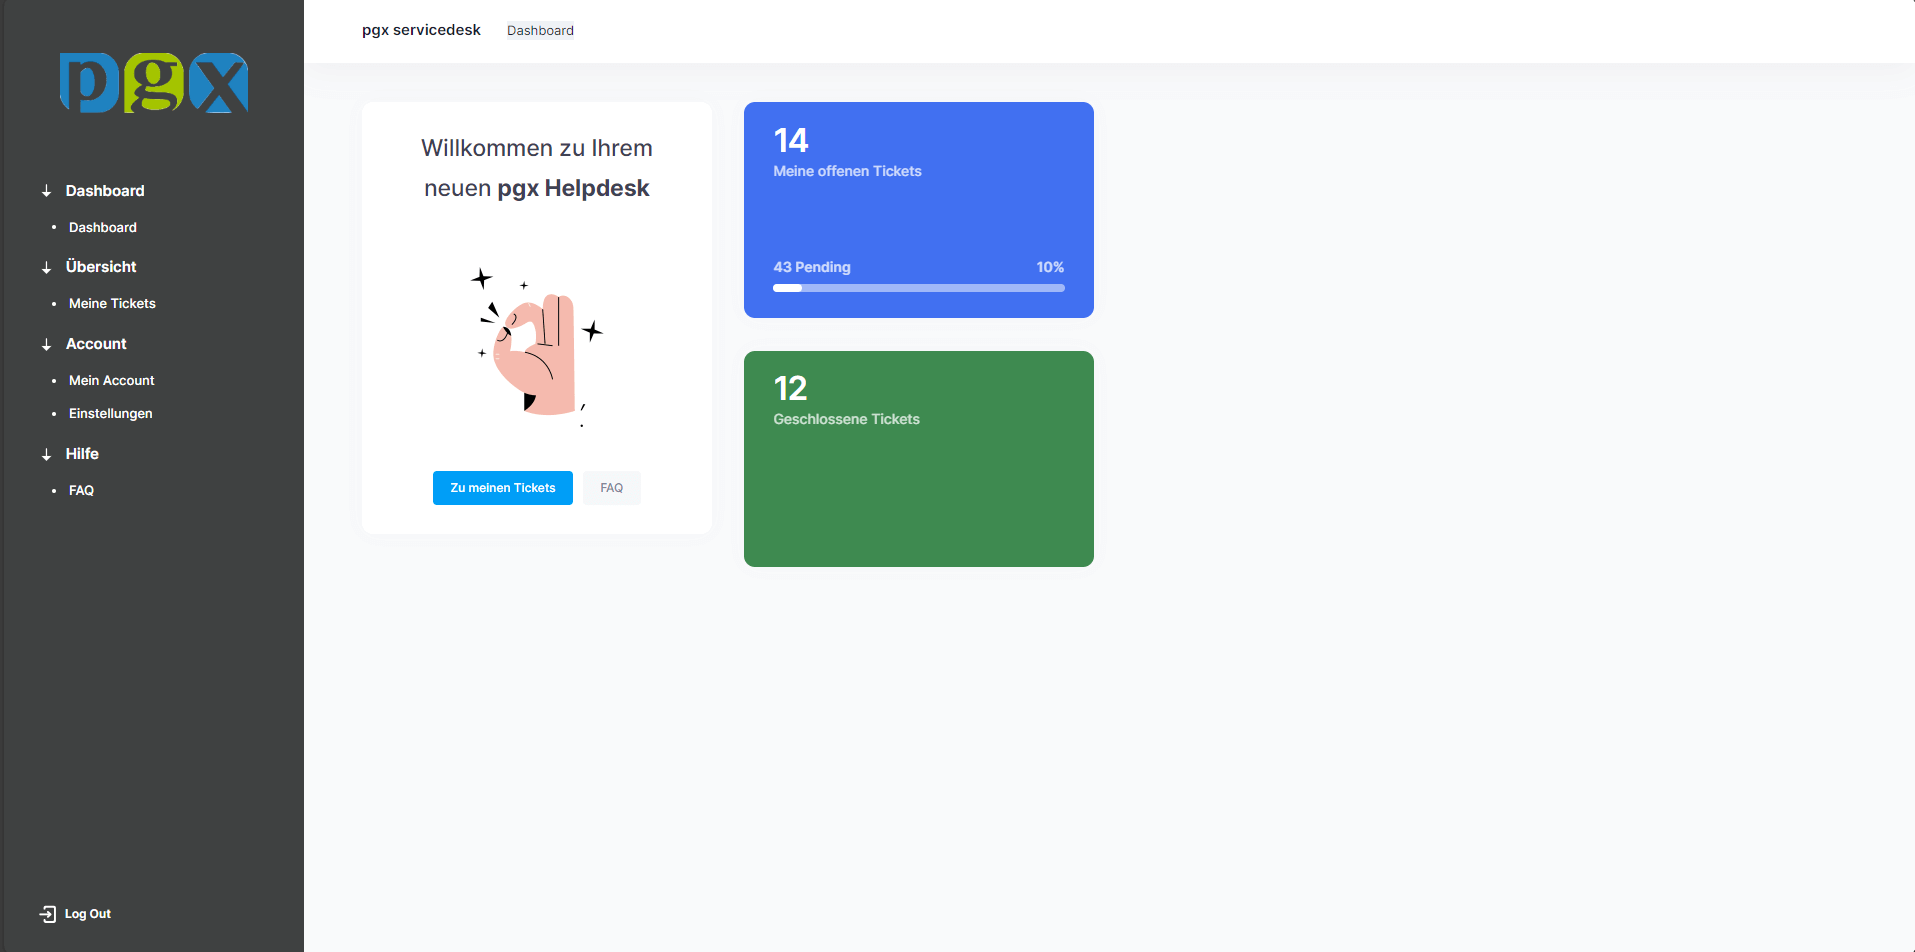
\includegraphics[width=\paperwidth,height=\paperheight]{UiB-images/mockups/dashboard_cropped.png}}
  \setbeamertemplate{navigation symbols}{}
  \begin{frame}[plain]
  \end{frame}
}
%%%%%%%%%%%%%%%%%%%%%%%%%%%%%%%%%%%%%%%%%%%%%%%%%%%%%%%%%%%%%%%%%% - KAP.4.3
% Kap.4 - Design - Wizard - 4.3
\subsection{Ticket-Wizard}
\SubSectionPage
{
  \usebackgroundtemplate{
\includegraphics[width=\paperwidth,height=\paperheight]{UiB-images/mockups/Wizard.pdf}}
  \setbeamertemplate{navigation symbols}{}
  \begin{frame}[plain]
  \end{frame}
  \addtocounter{framenumber}{-1}
}
{
  \usebackgroundtemplate{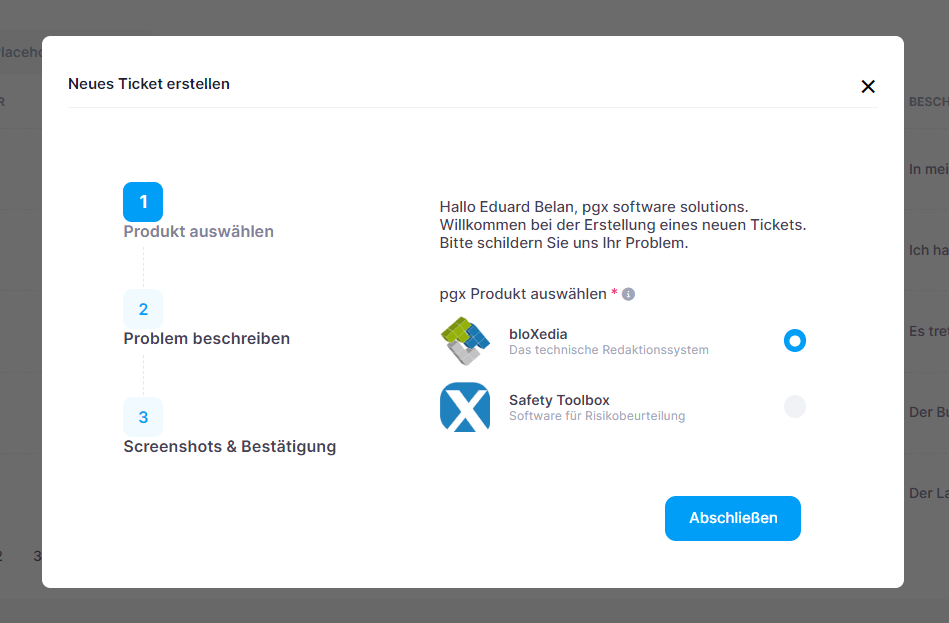
\includegraphics[width=\paperwidth,height=\paperheight]{UiB-images/mockups/wiz_1.png}}
  \setbeamertemplate{navigation symbols}{}
  \begin{frame}[plain]
  \end{frame}
}
%%%%%%%%%%%%%%%%%%%%%%%%%%%%%%%%%%%%%%%%%%%%%%%%%%%%%%%%%%%%%%%%%%%% - KAP.5
% Kap.5 - Technische Umsetzung
\section{Technische Umsetzung}
\begin{frame}{Inhaltsverzeichnis}
  \vspace{3em}
  \hspace{1em}
  \begin{minipage}{0.48\textwidth}
    {\small
      \tableofcontents[sections={1-3}, currentsection]
    }
  \end{minipage}
  \hfill
  \begin{minipage}{0.48\textwidth}
    {\small
      \tableofcontents[sections={4-7}, currentsection]
    }
  \end{minipage}
\end{frame}
%\SectionPage
%%%%%%%%%%%%%%%%%%%%%%%%%%%%%%%%%%%%%%%%%%%%%%%%%%%%%%%%%%%%%%%%%% - KAP.5.1
% Kap.5 - Technische Umsetzung - Architektur & Tech-Stack - 5.1
\subsection{Architektur}
\foreach \x in {0,...,18} {
  \usebackgroundtemplate{\includegraphics[width=\paperwidth,height=\paperheight]{UiB-images/architecture_and_tech_stack/ar_\x.png}}
  \setbeamertemplate{navigation symbols}{}
  \begin{frame}[plain]
  \end{frame}
  \addtocounter{framenumber}{-1}
}
\subsection{Tech-Stack}
\addtocounter{framenumber}{+1}
%%%%%%%%%%%%%%%%%%%%%%%%%%%%%%%%%%%%%%%%%%%%%%%%%%%%%%%%%%%%%%%%%%%% - KAP.6
% Kap.6 - Retrospektive
\section{Retrospektive}
\begin{frame}{Inhaltsverzeichnis}
  \vspace{3em}
  \hspace{1em}
  \begin{minipage}{0.48\textwidth}
    {\small
      \tableofcontents[sections={1-3}, currentsection]
    }
  \end{minipage}
  \hfill
  \begin{minipage}{0.48\textwidth}
    {\small
      \tableofcontents[sections={4-7}, currentsection]
    }
  \end{minipage}
\end{frame}
%\SectionPage
%%%%%%%%%%%%%%%%%%%%%%%%%%%%%%%%%%%%%%%%%%%%%%%%%%%%%%%%%%%%%%%%%% - KAP.6.1
% Kap.6 - Retrospektive - Selbstreflexion - 6.1
\subsection{Selbstreflexion}
\foreach \x in {1,...,5} {
  \usebackgroundtemplate{\includegraphics[width=\paperwidth,height=\paperheight]{UiB-images/retro/retro_\x.pdf}}
  \setbeamertemplate{navigation symbols}{}
  \begin{frame}[plain]
  \end{frame}
  \addtocounter{framenumber}{-1}
}
%%%%%%%%%%%%%%%%%%%%%%%%%%%%%%%%%%%%%%%%%%%%%%%%%%%%%%%%%%%%%%%%%%%% - KAP.7
% Kap.7 - Back to the Future
\section{Ausblick}
\addtocounter{framenumber}{+1}
\begin{frame}{Inhaltsverzeichnis}
  \vspace{3em}
  \hspace{1em}
  \begin{minipage}{0.48\textwidth}
    {\small
      \tableofcontents[sections={1-3}, currentsection]
    }
  \end{minipage}
  \hfill
  \begin{minipage}{0.48\textwidth}
    {\small
      \tableofcontents[sections={4-7}, currentsection]
    }
  \end{minipage}
\end{frame}
%\SectionPage
%%%%%%%%%%%%%%%%%%%%%%%%%%%%%%%%%%%%%%%%%%%%%%%%%%%%%%%%%%%%%%%%%% - KAP.7.1
% Kap.7 - Back to the Future - Doc & McFly - 7.1
\subsection{In die Zukunft}
{
  \usebackgroundtemplate{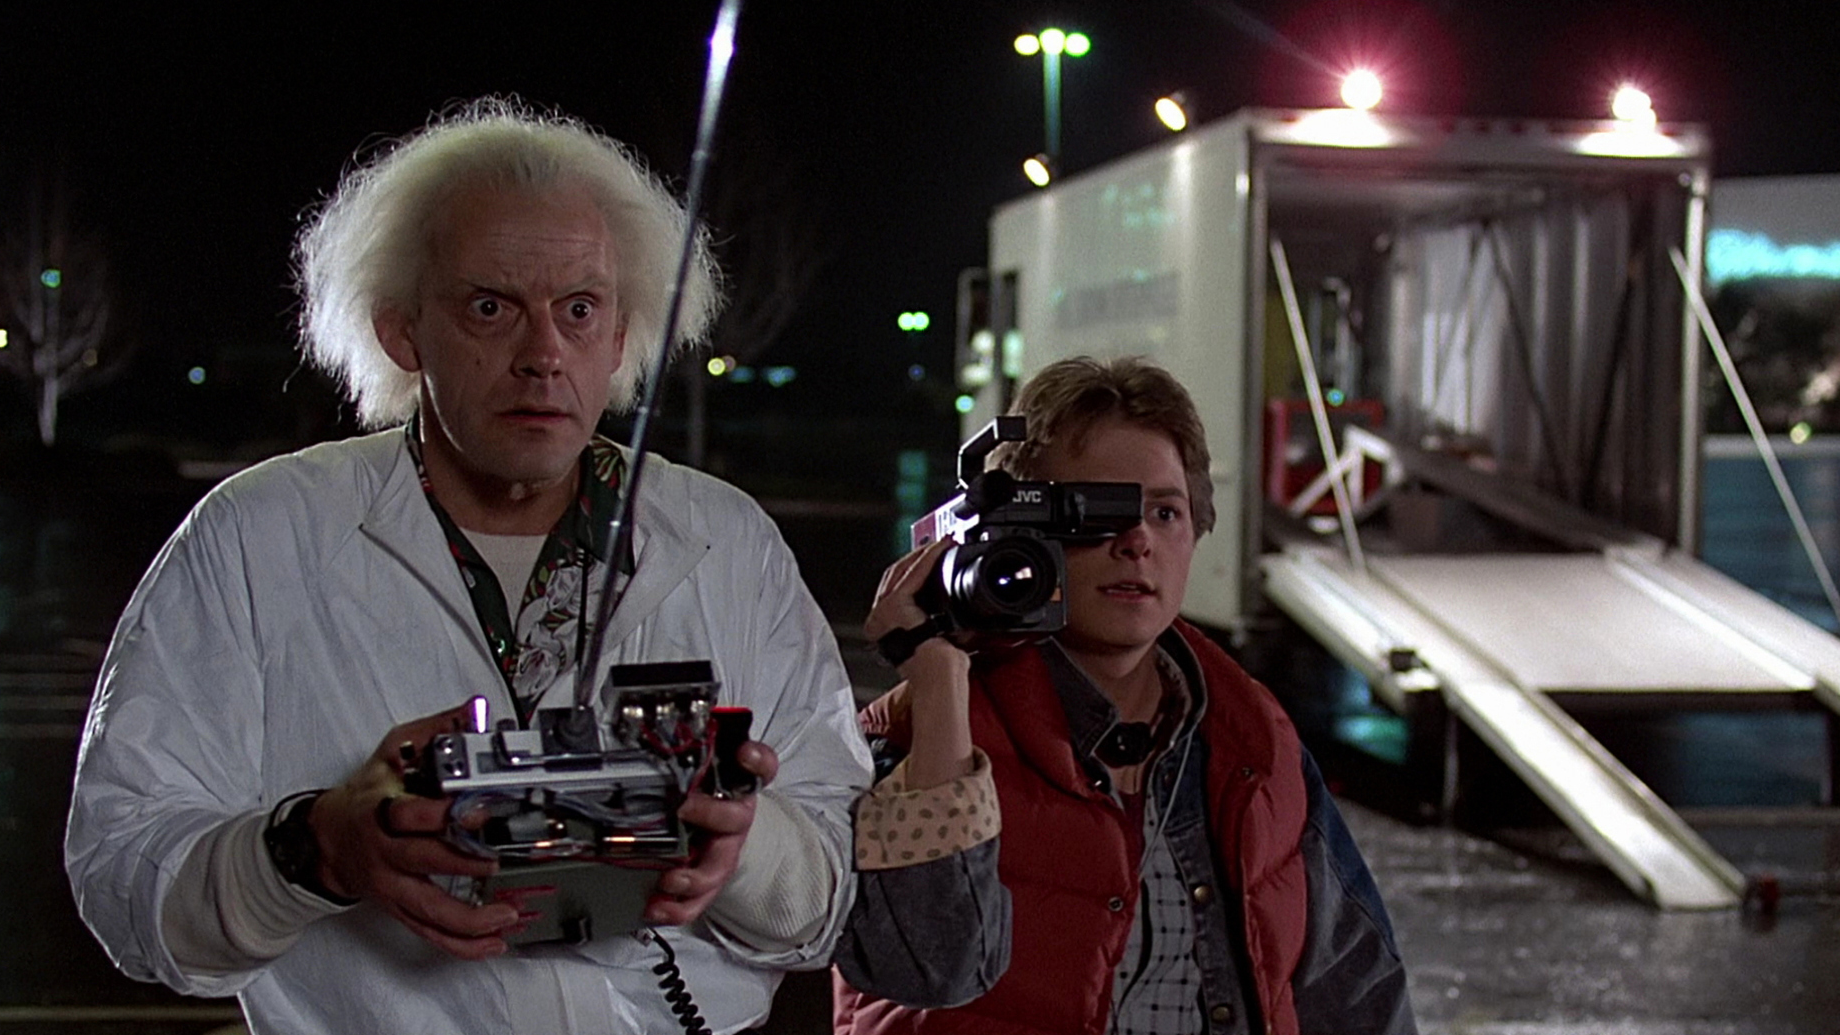
\includegraphics[width=\paperwidth,height=\paperheight]{UiB-images/bttf.png}}
  \setbeamertemplate{navigation symbols}{}
  \begin{frame}[plain]
  \end{frame}
}
%%%%%%%%%%%%%%%%%%%%%%%%%%%%%%%%%%%%%%%%%%%%%%%%%%%%%%%%%%%%%%%%%% - THANK YOU!
\subsection{}
{
  \usebackgroundtemplate{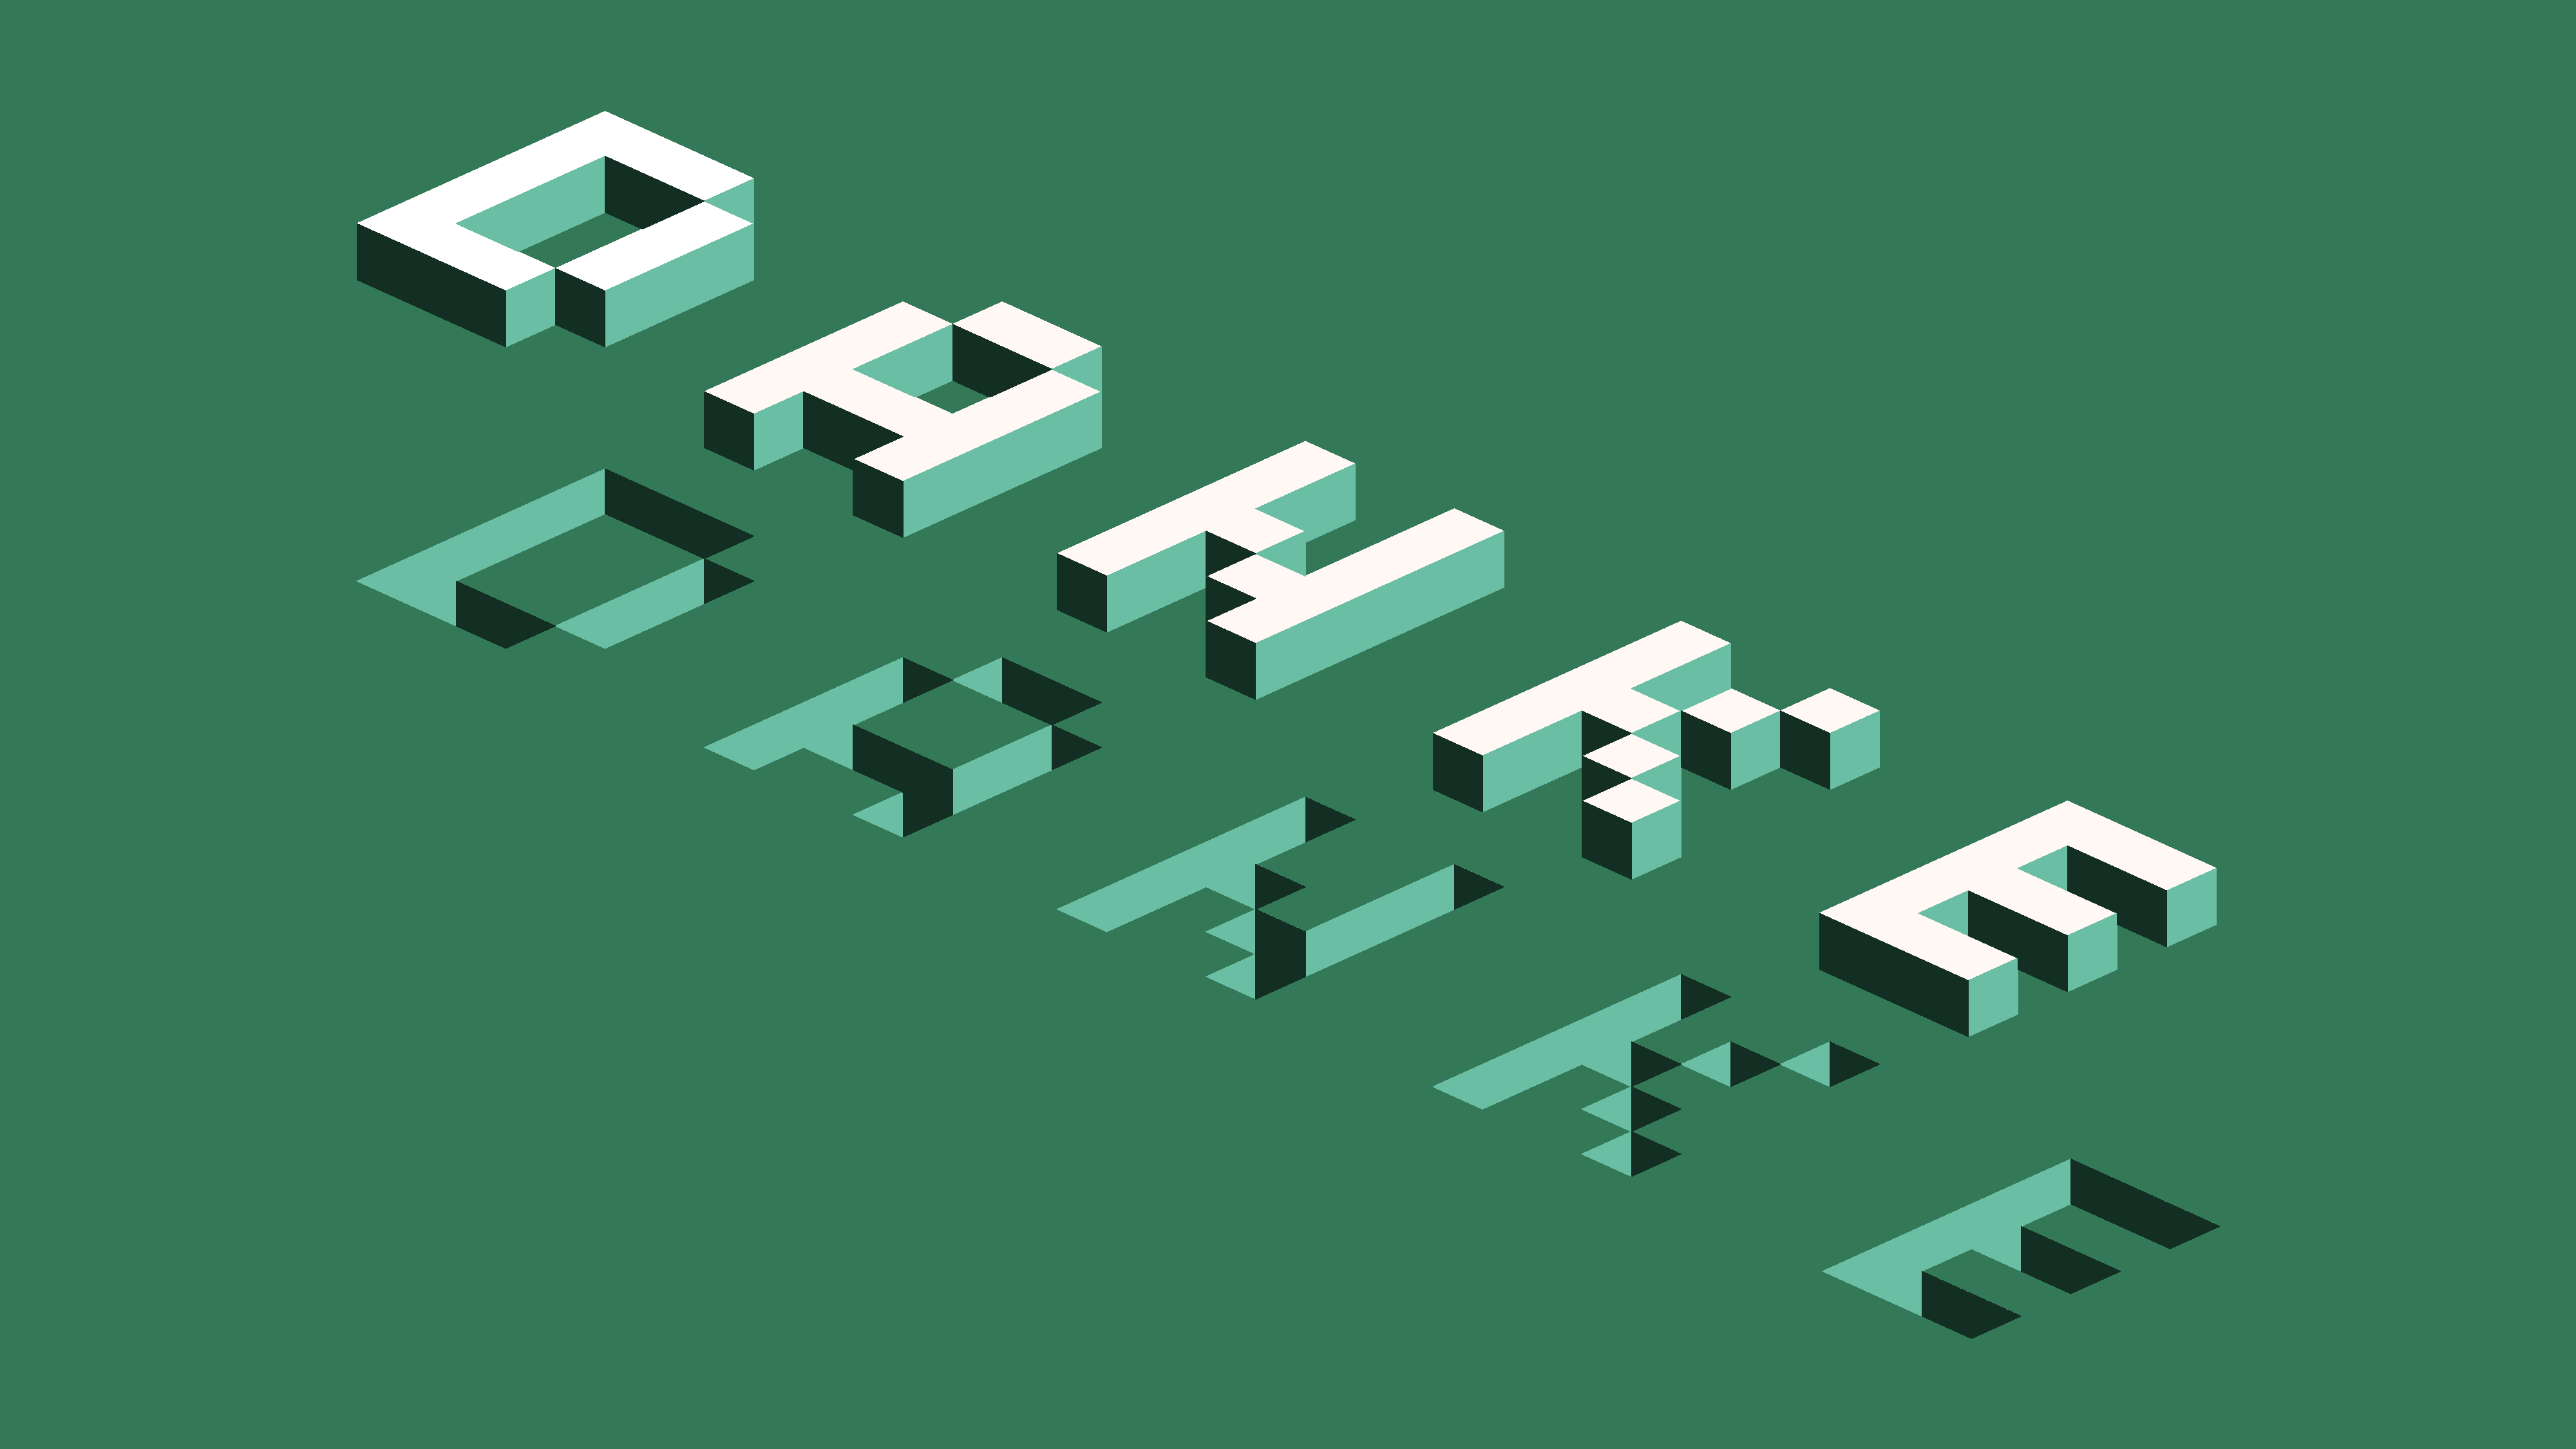
\includegraphics[width=\paperwidth,height=\paperheight]{UiB-images/ty.pdf}}
  \setbeamertemplate{navigation symbols}{}
  \begin{frame}[plain]
  \end{frame}
  \addtocounter{framenumber}{-1}
}
%%%%%%%%%%%%%%%%%%%%%%%%%%%%%%%%%%%%%%%%%%%%%%%%%%%%%%%%%%%%%%%%%% - DOC END
\end{document}